\documentclass[14pt]{extreport}
\usepackage[utf8]{vietnam}
\usepackage{indentfirst}
\usepackage{color}

\usepackage[utf8]{inputenc}
\usepackage[utf8]{vietnam}
\usepackage[vietnam]{babel}
\usepackage{verbatim}
\usepackage{csquotes}
%\usepackage{type1cm}
\usepackage[left=3.50cm, right=2.00cm, top=3.50cm, bottom=3.00cm]{geometry}
%\usepackage[left=3.0cm, right=1.50cm, top=3.00cm, bottom=2.50cm]{geometry}
\usepackage{graphicx}
\usepackage{multirow}
\usepackage{float}
\usepackage{mathrsfs} 
\usepackage{hyperref}
\usepackage{amsfonts}
\usepackage{longtable}
\usepackage[intlimits]{amsmath}
\usepackage{rotating}
\usepackage{array}
\usepackage{multirow}
\usepackage{mathtools} 
\usepackage{amsxtra,amssymb,latexsym,amscd,amsthm}
\usepackage{algorithm}
\usepackage[noend]{algpseudocode}
\usepackage{subfigure}

\newtheorem{theorem}{\MakeUppercase{Đ}ịnh lý}[chapter]
\newtheorem{corrollary}{\MakeUppercase{H}ệ quả}[chapter]
\newtheorem{definition}{\MakeUppercase{Đ}ịnh nghĩa}[chapter]
\newtheorem{clause}{\MakeUppercase{M}ệnh đề}[chapter]
\newtheorem{thuattoan}{\MakeUppercase{T}huật toán}[chapter]
% khoảng cách dòng 1.5 lines (như trong MS Word)
\renewcommand{\baselinestretch}{1.5}

%——————–
\begin{document}
\numberwithin{equation}{section}
\pagenumbering{gobble}
%TẤT CẢ các đoạn trong văn bản đều thụt ra ngoài

 
\setlength{\parindent}{2em}
\setlength{\parskip}{1em}


\bgroup
\setlength{\parindent}{0px} 
%tao khung
\newcommand{\Khung}[2]{

\begin{tabular}{|l|}
\hline\rule[-2ex]{0pt}{5.5ex}
\parbox{#1}{#2}\\
\hline
\end{tabular}
}

\Khung{.92\textwidth}{

\begin{center}

\normalsize
\textbf{TRƯỜNG ĐẠI HỌC BÁCH KHOA HÀ NỘI}\\
\normalsize
\textbf{VIỆN TOÁN ỨNG DỤNG VÀ TIN HỌC}\\
\textbf{------------------------------------------------------}\\[0.4cm]

\includegraphics[scale=.2]{image/Logo_Hust.png}\\[1.2cm]

\textbf{{\large HỆ THỐNG PHÂN TÍCH THÔNG TIN TRONG VĂN BẢN TÀI CHÍNH SỬ DỤNG HỌC CHUYỂN TIẾP}}\\[1cm]
\textbf{{\large}}\\[1cm]
\textbf{{\large ĐỒ ÁN TỐT NGHIỆP ĐẠI HỌC
}}\\
\textbf{Chuyên ngành: {\large TOÁN TIN}}\\[0.2cm]
\end{center}
\begin{flushleft}
\hspace{0.5 cm} \textbf{ Hướng dẫn:{ TS. NGUYỄN THỊ THANH HUYỀN }}\\[0.2cm]
\hspace{0.5 cm} \textbf{ Thực hiện:\hspace{0.5cm}{NGUYỄN HỒNG SƠN}}\\
\hspace{0.5 cm} \textbf{ Lớp :\hspace{1.9 cm}{KSTN Toán tin K59}}\\

\end{flushleft}

\vspace{1.3cm}
\begin{center}
\textbf{{\large HÀ NỘI - 2019}}\\
\end{center}
}
\egroup



\chapter*{Danh mục từ viết tắt}
\addcontentsline{toc}{chapter}{{\bf Danh mục từ viết tắt}\rm}

\begin{tabular}{l l }

BERT & Bidirectional Encoder Representations from Transformers.\\

LSTM & Long short term memory\\

RNN & Recurent neural network\\

MLP & Multi-layer perceptron \\

BoW & Bag of Word \\

Tfidf &  Term frequency – inverse document frequency\\

HMMs & Hidden Markov Model \\

CRF & Conditional random field \\

MEMMS & Maximum Entropy Markov Models \\

acc & Accuracy \\

NER & Named entity recognition \\

ML & Machine learning \\
\end{tabular}
\newpage

% \listoffigures
\listoftables
% \chapter*{Danh mục hình vẽ, bảng biểu}
% \addcontentsline{toc}{chapter}{{\bf Danh mục hình vẽ, bảng biểu}\rm}

% \begin{tabular}{l l }

% Hình \ref{fig:classication_pipeline} & Luồng xử lý bằng học máy\\

% Hình \ref{fig:BoW} & Mô hình Bag of Word\\

% Hình \ref{fig:MLP} & Mô hình mạng neuron\\

% Hình \ref{fig:lstm} & Mô hình mạng bộ nhớ dài ngắn\\

% Hình \ref{fig:luong_attention} & Cơ chế attention tổng quát \\

% Hình \ref{fig:bahaunau_att} & Cơ chế attention cục bộ \\

% Hình \ref{fig:global_attention} & Cơ chế attention toàn cục \\

% Hình \ref{fig:Transformer} & Mô hình Transformer \\

% Hình \ref{fig:input_bert} & Biểu diễn dữ liệu đầu vào BERT \\

% Hình \ref{fig:sequence_labeling} & Mô hình gán nhãn tuần tự của Flair \\

% Hình \ref{fig:flair_lm} & Mô hình ngôn ngữ của Flair \\

% hình \ref{fig:sub1} & Báo cáo tài chính công ty thủy sản Mekong \\

% Hình \ref{fig:sub2} & Báo cáo tài chính công ty cổ phần Hóa An \\

% Bảng \ref{tab:ner} & Kết quả mô hình NER sử dụng Flair \\

% Hình \ref{fig:bert_cls} & Mô hình phân lớp câu văn sử dụng BERT \\
% \end{tabular}
% \newpage
% \begin{tabular}{l l }
% Bảng \ref{tab:cls} & Kết quả mô hình phân lớp câu văn sử dụng BERT \\

% Hình \ref{fig:input_doc} & Văn bản dữ liệu đầu vào hệ thống \\

% Hình \ref{fig:output} & Giao diện kết quả \\

% Hình \ref{fig:read} & Kết quả đọc văn bản \\

% Hình \ref{fig:extract} & Kết quả trích xuất thông tin \\

% Hình \ref{fig:analysis} & Kết quả phân tích thông tin
% \end{tabular}

\tableofcontents

%\listoffigures

\newpage
\setcounter{page}{1}
\pagenumbering{arabic}
\addcontentsline{toc}{chapter}{{\bf Mở đầu}}

\chapter*{Mở đầu}
 \textbf{Lý do chọn đề tài}\\
 
Bài toán trích chọn và phân tích thông tin trong văn bản đã và đang được tiếp cận và khai thác theo nhiều hướng khác nhau. Trong đó phổ biến là các phương phương pháp học sâu dựa trên những bộ dữ liệu lớn và đã ghi nhận những kết quả tốt với tính tổng quát cao. Tuy nhiên đối với những bài toán thực tế, tập dữ liệu huấn luyện không sẵn có và tốn rất nhiều chi phí để tạo ra, cần phải có những phương pháp tiếp cận tập trung vào việc khai thác được đặc trưng ngôn ngữ từ những bộ dữ liệu có kích thước nhỏ hoặc khai thác thông tin từ các tập dữ liệu lớn và sử dụng thông tin học được áp dụng lên bài toán cụ thể. Một dạng văn bản đặc trưng đó là các văn bản tài chính chứa đựng nhiều thông tin quan trọng liên quan đến tình hình tài chính của công ty. Tuy nhiên, đây là các văn bản đặc trưng nên dữ liệu có sẵn là không có nhiều, điều này đặt ra những thách thức lớn đối với các mô hình trí tuệ nhân tạo thông thường trong việc huấn luyện. Mặc khác lợi ích đem đến từ việc phân tích những báo cáo tài chính là là rất to lớn. Do đó, em mạnh dạn chọn đề tài \textbf{"Hệ thống phân tích thông tin trong văn bản tài chính sử dụng học chuyển tiếp"} với mục đích đưa ra một phương pháp trích chọn và phân tích thông tin từ văn bản tài chình, với tập dữ liệu huấn luyện nhỏ nhưng vẫn đạt được những kết quả khả quan.

\textbf{Đối tượng và phạm vi nghiên cứu}\\
Trong báo cáo này, em tập trung nghiên cứu:
\begin{itemize}
    \item Tập dữ liệu bao gồm một số lượng nhỏ các văn bản dạng báo cáo tài chính của nhiều công ty sử dụng ngôn ngữ Tiếng Việt.
    \item Bài toán trích lọc và phân tích thông tin.
    \item Các phương pháp học chuyển tiếp
    \item Áp dụng phương pháp học chuyển triếp trên tập dữ liệu là các văn bản tài chính, ưu và nhược điểm
\end{itemize}

\textbf{Ý nghĩa khoa học và thực tiễn của đề tài}\\
Ý nghĩa khoa học của đề tài là đánh giá phương pháp học chuyển tiếp đối với dữ liệu cụ thể là tiếng việt, thực hiện trích chọn và phân tích thông tin từ các báo cáo tài chính với mục đích chọn lọc ra những thông tin quan trọng và đánh giá bước đầu dựa trên ngữ cảnh cụ thể của văn bản trong điều kiện tập dữ liệu huấn luyện hạn chế. Đề tài này có ứng dụng thực tiễn rất lớn khi mà nhu cầu phân tích thông tin trong các văn bản tài chính là rất lớn, trong khi tập dữ liệu huấn luyện cho các loại văn bản đặc thù này cần rất nhiều chi phí để tạo ra, do đó thường có kích thước nhỏ. 

\textbf{Cấu trúc báo cáo}\\
Báo cáo này được trình bày theo ba chương:
\begin{itemize}
    \item Chương thứ nhất trình bày các bài toán liên quan đến vấn đề trích chọn và đánh giá thông tin trong văn bản nói chung cũng như bài toán trích chọn thông tin trong báo cáo tài chính. Các bài toán này bao gồm nhận diện thực thể tên và phân lớp câu văn. Những hướng tiếp cận hiện tại cho từng bài toán này cũng được giới thiệu và phân tích ưu và nhược điểm của từng phương pháp tiếp cận
    \item Chương thứ hai trình bày cụ thể về mô hình học chuyển tiếp (Transfer learning), trong đó có mạng biểu diễn hai chiều tiền huấn luyện cho mô hình ngôn ngữ ( BERT) và mô hình biểu diễn ngôn ngữ dựa trên ngữ cảnh dành cho mô hình dán nhãn tuần tự ( Flair). Đây là những mô hình ngôn ngữ đem lại kết quả rất tốt và đã được kiểm chứng là đem lại kết quả tốt nhất cho nhiều tác vụ xử lý ngôn ngữ tự nhiên.
    \item Chương thứ ba là cách thức triển khai và áp dụng mô hình vào bài toán trích chọn và phân tích thông tin trong văn bản tài chính. Đưa ra các phân tích, đánh giá và kết luận về kết quả của hệ thống, hiệu quả của mô hình, tiềm năng ứng dụng trong thực tế.
\end{itemize}

\chapter*{Lời cảm ơn}
Em xin gửi những lời cảm ơn chân thành nhất tới \textbf{ TS. Nguyễn Thị Thanh Huyền} , người đã trực tiếp hướng dẫn em hết sức tận tình, chu đáo về mặt chuyên môn, động viên em về mặt tinh thần để em hoàn thành bản đồ án tốt nghiệp này.

Em xin gửi lời cảm ơn tới tất cả thầy cô giáo trong Viện Toán Ứng Dụng và Tin Học, Trường Đại Học Bách Khoa Hà Nội đã tận tình dạy dỗ, chỉ bảo em trong suốt thời gian năm năm học tập và rèn luyện tại trường.

Em cũng xin gửi lời cảm ơn đến các anh chị và đồng nghiệp tại Công ty TNHH Cinnamon, Công ty cổ phần giải pháp và nguồn lực công nghệ ITSOL và Trung tâm Công nghệ mạng Viettel đã cho phép em thực tập và làm việc, hướng dẫn và chỉ bảo những kinh nghiệm quý báu.

Em xin gửi lời cảm ơn tới tất cả bạn bè trong lớp KSTN Toán Tin K59 đã hộ trợ, đồng hành, cùng phấn đấu và cố gắng cùng trong suốt quãng thời gian dài học tập tại trường. Sự giúp đỡ của các bạn là vô cùng lớn lao.

Cuối cùng cùng em xin gửi lời cảm ơn tới gia đình, người thân và bạn bè đã luôn động viên giúp đỡ em trong suốt quá trình học tập tại Trường Đại Học Bách Khoa Hà Nội cũng như trong thời gian thực hiện đồ án tốt nghiệp.

Hà Nội, Ngày 21 Tháng 05 Năm 2019

Sinh viên

Nguyễn Hồng Sơn


\chapter{Tổng quan bài toán}

\section{Trích chọn thông tin trong văn bản}
Trích chọn thông tin trong văn bản là một lĩnh vực nhỏ trong xử lý ngôn ngữ tự nhiên có tính ứng dụng cao và có nhu cầu cấp thiết trong thực tế. Trích chọn thông tin (thu thập thông tin) được định nghĩa như sau:
\begin{definition}
Trích chọn thông tin (Information retrieval - IR) nghiên cứu tác vụ trích chọn tự động thông tin có cấu trúc từ dữ liệu mà máy tính có thể đọc được. Đối với dữ liệu xử lý là các văn bản, bài toán trở thành một lĩnh vực của xử lý ngôn ngữ tự nhiên. 
\end{definition}
Đây là một lĩnh vực khó nên hầu hết các phương pháp tiếp cận hiện tại đều tập trung vào những tập dữ liệu cụ thể để khai thác các thông tin và đặc điểm từ tập dữ liệu, từ đó đưa ra phương pháp tiếp cận phù hợp.

Dựa vào đặc điểm của thông tin cần được tách ra mà bài toán được chia thành các bài toán nhỏ hơn như sau:
\begin{itemize}
    \item Tìm kiếm trong mẫu (Template filling)
    \item Nhận diện thực thể tên (Named entity recognition - NER)
    \item Phân tích mối liên hệ giữa các thông tin (Relationship extraction)
    \item Trích chọn thông tin có cấu trúc
    \begin{itemize}
        \item Trích chọn trường thông tin trong bảng
        \item Trích chọn câu văn, đoạn văn
    \end{itemize}
\end{itemize}

\subsection{Nhận diện thực thể tên}
Nhận dạng thực thể có tên (Named Entity Recognition – NER)(còn gọi là nhận dạng thực thể định danh, xác định thực thể hoặc trích xuất thực thể) nhằm nhận biết các chuỗitừ trong văn bản là tên của một đối tượng nào đó, điển hình như:  

\begin{itemize}
    \item Tên người (Person) 
    \item Tên tổ chức (Organization)
    \item Tên địa điểm (Location) 
    \item Thời gian (Datetime) 
    \item Tiền tệ (Monetary)
    \item Phần trăm (Percentage) 
\end{itemize}

Trong đó, có các thực thể như thời gian, tiền tệ và phần trăm thường ít mang tính nhập nhằng, không khó để nhận dạng. Các thực thể khác như tên người, tên tổ chức, tên địa điểm thường mang tính nhập nhằng, phải dựa vào ngữ cảnh của câu để xác định tốt hơn. Ngoài ra, trong từng lĩnh vực cụ thể, chúng ta cần thêm vào các loại thực thể đặc thù. Ví dụ, trong lĩnh vực y tế cần xác định thêm thực thể loại bệnh và loại thuốc, trong lĩnh vực sinh học cần định nghĩa thêm các thực thể gen mang bệnh,...

Về mặt toán học, bài toán được định nghĩa như sau: cho trước tập các chuỗi quan sát ký hiệu $\textbf{x} = (x_1, x_2, ...,x_n)$. Thông thường $x_i$ được biểu diễn dưới dạng vector. Ta mong muốn gán nhãn $y_i$ dựa vào dữ kiện từ các $x_i$ trước đó.\\
Để gán nhãn, ta thường dùng BIO notation (trước đó dùng trong text chunking). Với mỗi entity kiểu T, ta có hai nhãn B-T và I-T. B-T là begin type T, I-T là inside type T. Ngoài ra, ta còn có nhãn O cho biết outside name entity. Ta có thể tham khảo ví dụ bên dưới.
\begin{displayquote}
Steve Jobs was a co-founder of Apple Inc\\
B-PER I-PER O O O O B-ORG I-ORG
\end{displayquote}

Là một bài toán khá quan trọng và được nghiên cứu khá rộng, nhưng hiện nay vẫn chưa có nhiều nghiên cứu cho bài toán này được áp dụng cho việc xử lý văn bản tiếng Việt. Ngoài ra các nghiên cứu hiện tại đang rất nhỏ, mang tính hàn lâm hoặc đóng kín trong nội bộ các công ty. Chính vì vậy chúng tôi quyết định đi sâu nghiên cứu, xây dựng một mô hình mạng nơ ron hồi quy cho kết quả tốt trên tiếng Việt, hơn nữa áp dụng mô hình này vào một bài toán thực tế có nhiều ứng dụng, bài toán trích xuất thông tin trên sơ yếu lý lịch (Curriculum Vitae - CV).

\subsection{Phân loại câu văn}
Bài toán phân loại văn bản - text classification là một trong những bài toán cơ bản và quan trong nhất của xử lý ngôn ngữ tự nhiên. Mục đích của bài toán là gán nhãn cho mỗi văn bản nói chung (cụ thể hơn là các câu văn, đoạn văn) nhãn tương ứng với ngữ nghĩa của bản thân câu văn, đoạn văn đó. Trên thực tế, đây là một bài toán được ứng dụng rất rộng rãi trong nhiều ứng dụng của xử lý ngôn ngữ tự nhiên như:
\begin{itemize}
    \item Đánh giá tính tích cực, tiêu cực được thể hiện trong câu văn
    \item Phát hiện mục đích của người nói, viết dựa trên nội dung của câu văn
    \item Khái quát nội dung của câu văn
\end{itemize}
Đây là một bài toán được nghiên cứu rất rộng rãi vì ý nghĩa thực tiễn cao do đó đã có rất nhiều phương pháp tiếp cận đối với bài toán này. Trong khuôn khổ luận văn này, em tập trung nghiên cứu hai bài toán phân lớp câu văn nhằm đánh giá tính tích cực, tiêu cực của câu văn. Việc thực hiện phân lớp được tiếp cận bằng cách sử dụng mô hình học chuyển tiếp.\\
Các phương pháp được lựa chọn tương ứng cho các bài toán nhằm giải quyết các thách thức riêng, tuy nhiên, về mặt tổng thể, các bài toán đều có những thách thức chung được thể hiện sau đây.

\section{Bài toán trích chọn thông tin trong văn bản tài chính}
\subsection{Văn bản tài chính}
Văn bản tài chính là văn bản chứa đựng  các thông tin về tình hình tài chính, tình hình kinh doanh và các luồng tiền của doanh nghiệp đáp ứng các cầu cho những người sử dụng chúng trong việc đưa ra các quyết định về kinh tế.

Văn bản, báo cáo tài chính phải cung cấp những thông tin của một doanh nghiệp về:
\begin{itemize}
    \item Các thông tin cơ bản của doanh nghiệp
    \item Tài sản
    \item Nợ phải trả
    \item Vốn chủ sở hữu
    \item Doanh thu, thu nhập khác, chi phí sản xuất kinh doanh và chi phí khác
    \item Lãi, lỗ và phân chia kết quả kinh doanh
    \item Các luồng tiền
\end{itemize}
Hình \ref{fig:sub1} là ví dụ về các thông tin cơ bản của doanh nghiệp trong một báo cáo tài chính.
\begin{figure}
\centering
  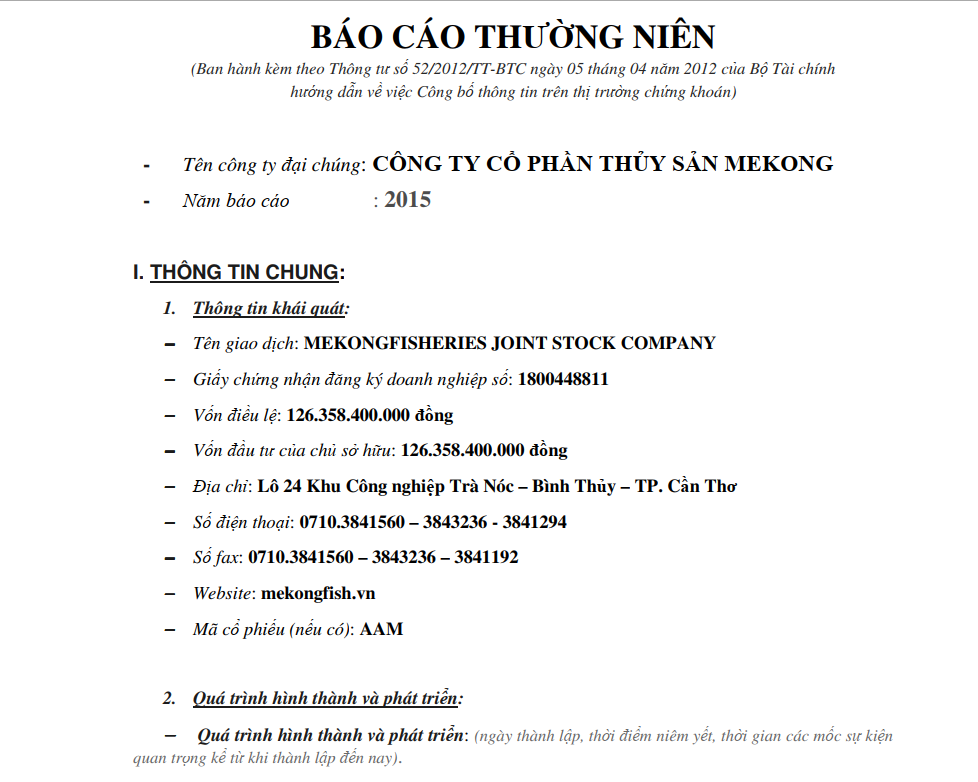
\includegraphics[width=1\linewidth]{image/baocao1.PNG}
  \caption{Báo cáo tài chính công ty thủy sản Mekong}
  \label{fig:sub1}
\end{figure}


\subsection{Đặc trưng dữ liệu}
Dữ liệu được sử dụng ở đây là tập hợp các câu văn, đoạn văn được lấy ra từ văn bản tài chính, cụ thể hơn là các báo cáo tài chính ở các định dạng có thể đọc trực tiếp không qua can thiệp bằng các phương pháp xử lý khác như nhận diện ký tự quang học, xử lý ảnh,... Các văn bản được sử dụng cho huấn luyện và đánh giá được chọn ngẫu nhiên từ tập 50 văn bản báo cáo tài chính của các công ty khác nhau. Đặc trưng của các văn bản này là không có định dạng cụ thể, các văn bản khác nhau được trình bày theo những quy tắc khác nhau thông tin cso thể nằm rải rác trong văn bản, không có những quy định cụ thể nào về việc trình bày thông tin. Ví dụ ở \ref{fig:sub2} là một báo cáo tài chính khác.
\begin{figure}
\centering
  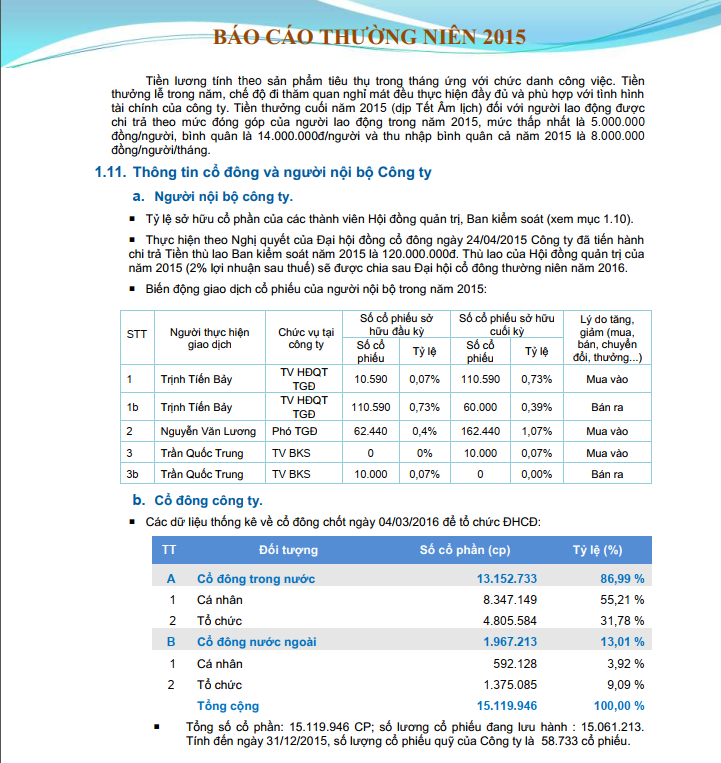
\includegraphics[width=1\linewidth]{image/baocao2.PNG}
  \caption{Báo cáo tài chính công ty cổ phần Hóa An}
  \label{fig:sub2}
\end{figure}
Các văn bản này bao gồm nhiều ảnh, biểu đồ, bảng, trong đó các bảng có thể là bảng ngang hoặc bảng dọc (header của bảng có thể nằm ở phía trên hoặc hai bên). Mặc dù việc xử lý thông tin trong bảng là rất quan trọng nhưng hệ thống không đặt vấn đề quá lớn vào việc xử lý bảng do để làm tốt điều này cần kết hợp rất nhiều các công nghệ khác nhau.

\subsection{Mục tiêu và thách thức}
Hệ thống tiếp cận và xử lý các văn bản báo cáo tài chính, đây là các văn bản phức tạp, có kích thước lớn nhưng chứa đựng nhiều thông tin quan trọng. Việc xử lý các văn bản báo cáo tài chính đem lại nhiều lợi ích to lớn đối với việc phân tích và đánh giá tình trạng hoạt động của một công ty, hỗ trợ đưa ra những quyết định quan trọng. Việc phân tích và đánh giá các văn bản tài chính chủ yếu tập trung vào phân tích và đánh giá các thông tin quan trọng như:
\begin{itemize}
    \item Đánh giá khái quát tình hình tài chính.
    \item Phân tích tình hình huy động và sử dụng vốn của doanh nghiệp (phân tích kết cấu và sự biến động của tài sản, nguồn vốn).
    \item Phân tích tình hình tài trợ và mức độ đảm bảo vốn cho hoạt động kinh doanh. 
    \item Phân tích tình hình công nợ và khả năng thanh toán.
    \item Phân tích khả năng tạo tiền và tình hình lưu chuyển tiền tệ.
    \item Phân tích tình hình và kết quả kinh doanh của doanh nghiệp.
    \item Phân tích điểm hoà vốn và việc ra quyết định.
    \item Phân tích hiệu suất và hiệu quả sử dụng vốn.
    \item Phân tích rủi ro tài chính và dự báo nhu cầu tài chính.
\end{itemize}
Đây là những nhu cầu thực tế đến từ nhiều đối tượng khác nhau như:
\begin{itemize}
    \item Nhà quản lý doanh nghiệp
    \item Nhà đầu tư
    \item Nhà cung cấp tín dụng
    \item Người hưởng lương trong doanh nghiệp
    \item Các cơ quan quản lý nhà nước
    \item ...
\end{itemize}
Tuy nhiên, việc phân tích các văn bản, báo cáo tài chính để đạt được sự hiệu quả và đáng tin cậy thì hàm lượng chuyên gia đưa vào rất cao, do đó việc tiếp cận và xử lý từng khía cạnh chi tiết, đánh giá cụ thể theo từng mục tiêu đã liệt kê ở trên yêu cầu một hệ thống xử lý đồng bộ với hàm lượng chuyên gia lớn. Do đó, hệ thống này  nhằm tiếp cận bước đầu đến quá trình xử lý bài toán bao:
\begin{itemize}
    \item Nhận diện, trích lọc và thu thập dữ liệu, số liệu.
    \item Xử lý, đánh giá bước đầu dữ liệu.
\end{itemize}
Cụ thể hơn, các thông tin được trích chọn ra bao gồm:
\begin{itemize}
    \item Thông tin về công ty:
    \begin{itemize}
        \item Tên công ty
        \item Địa chỉ
    \end{itemize}
    \item Thông tin về người:
    \begin{itemize}
        \item Tên
        \item Ngày sinh
        \item Giới tính
        \item Địa chỉ
        \item Vị trí
    \end{itemize}
\end{itemize}
Việc đánh giá sơ bộ là đánh giá một số mặt về các thông tin của một câu văn cụ thể. Các câu văn này gắn liền với những thông tin quan trọng được nhắc tới như:
\begin{itemize}
    \item Nợ
    \item Doanh thu
    \item Lợi nhuận
    \item Vốn
    \item Chi phí
\end{itemize}
Các đánh giá bao gồm:
\begin{itemize}
    \item Trạng thái của thông tin được nhắc đến:
    \begin{itemize}
        \item Tích cực
        \item Tiêu cực
        \item Trung tính
    \end{itemize}
    \item Thời điểm thông tin được nhắc đến
    \begin{itemize}
        \item Quá khứ
        \item Hiện tại
        \item Tương lai
    \end{itemize}
\end{itemize}
Các đánh giá này hoàn toàn dựa vào nội dung của chính câu văn đó.


Mặc dù mang lại rất nhiều thông tin nhưng vì văn bản tài chính là các loại văn bản rất đặc thù, điều đó đem lại rất nhiều thách thức đối với việc trích chọn cũng như phân tích thông tin. Việc đi sâu phân tích và đánh giá ý nghĩa của từng thông tin trong văn bản là vô cùng khó khăn, do đó phương pháp tiếp cận hiện tại chỉ mang tính tổng quan, trích chọn và đưa ra những đánh giá tương đối tổng thể về thông tin trong văn bản tài chính. Mặt khác, việc xử lý văn bản trong tiếng Việt cũng có những thách thức chung như sau:
\begin{itemize}
    \item Tiếng Việt mang nhiều đặc trưng ngôn ngữ phức tạp, từ nhiều nghĩa, mang tính nhập nhằng khá nhiều và khác biệt cấu trúc ngữ pháp so với tiếng Anh, do đó việc áp dụng hoàn toàn mô hình tiếng Anh là không thể. 
    \item Chưa có bộ dữ liệu đầy đủ nào được công bố cho tiếng Việt cho việc áp dụng và đánh giá mô hình tốt hơn.
    \item Chưa có nhiều nghiên cứu tiền đề trong vấn đề nhận dạng thực thể tiếng Việt.
    \item Chưa có một mô hình tổng quát cho các bài toán phân lớp văn bản nói chung, và phân lớp câu trong tiếng Việt nói riêng.
\end{itemize}
Yếu tố tiếp theo là về mặt dữ liệu của bài toán này. Văn bản tài chính là các văn bản dài do đó việc tạo dữ liệu huấn luyện yêu cầu chi phí rất lớn, mặt khác số lượng văn bản lại không hề lớn vì đây là các văn bản rất đặc thù, do đó mặc dù tiếp cận bài toán dưới góc độ xử lý từng câu văn, thì vẫn có hai vấn đề lớn:
\begin{itemize}
    \item Tập dữ liệu huấn luyện nhỏ
    \item Ngữ cảnh của các câu văn rất đa dạng
\end{itemize}
Về mặt định dạng văn bản, các văn bản này mặc dù có cấu trúc là các báo cáo, tuy nhiên tất cả đều chỉ thỏa mãn các yêu cầu tổng quát về mặt kiến trúc một bản báo cáo tài chính. Đối với từng văn bản khác nhau lại không có một quy định cụ thể về cách thức trình bày, do đó đặt ra rất nhiều thách thức cho việc xử lý.
 


\section {Các hướng tiếp cận thông thường}
Hệ thống đi giải quyết hai bài toán cho các vấn đề tương ứng là:
\begin{itemize}
    \item Bài toán nhận diện thực thể tên giải quyết vấn đề trích xuất thông tin
    \item Bài toán phân lớp câu văn giải quyết vấn đề đánh giá câu văn
\end{itemize}
Mỗi bài toán sẽ có các mô hình riêng đã được chứng minh là hiệu quả. Cụ thể hơn, tùy theo đặc trưng dữ liệu của từng bài toán mà có những mô hình đặc biệt tương ứng. Tuy nhiên, về mặt tổng quát, ta có thể chia các phương pháp giải quyết cho các bài toán nói trên theo bốn nhóm:
\begin{itemize}
    \item Các phương pháp sử dụng luật
    \item Các phương pháp học máy
    \item Các phương pháp học sâu
    \item Các phương pháp học chuyển tiếp
\end{itemize}
Mỗi phương pháp có những đặc điểm riêng phù hợp với từng hoàn cảnh cũng như đặc trưng của tập dữ liệu.

\subsection{Các phương pháp sử dụng luật}
Hướng tiếp cận sử dụng hệ luật được xây dựng bởi chuyên gia: Hướng tiếp cận này là hướng tiếp cận dễ nhất, có kết quả nhanh và đòi hỏi người sử dụng có kiến thức cao về thực thể cần trích xuất cũng như gan nhãn cho câu văn. Hơn nữa để tăng độ chính xác thì đòi hỏi lượng thời gian tạo luật mất thời gian, tính kế thừa ít. Hệ luật thường được tiếp cận bằng cách xem xét các vấn đề sau: Từ loại (danh từ, động từ,...), ngữ cảnh (từ đứng trước, từ đứng sau), thuộc tính riêng của thực thể (độ dài, viết hoa,...) kết hợp với bộ từ điển của thực thể để tạo luật. Ví dụ bài toán NER với câu sau đây: 
    \begin{displayquote}
    "President Bush said Monday's talk will incude discussion on security, a timetable for US forces to leave Iraq"
    \end{displayquote}
    Trong ví dụ này, từ "Bush" đứng sau từ "President" sẽ được nhận định là tên người (Person), "Iraq" đứng sau động từ "leave" sẽ được nhận định là tên địa điểm (Location).
    
\subsection{Các mô hình học máy}
Đối với bài toán nhận diện thực thể tên, có những mô hình học máy đem lại hiệu quả khá tốt như sau:
\begin{itemize}
\item Mô hình Markov ẩn (Hidden Markov Model – HMMs): Thuật toán này sử dụng Maximum Likelihood Estimation sao cho cực đại hóa xác suất p(\textbf{x}, \textbf{y}), trong đó \textbf{x} là tất cả các câu trong ngữ liệu, \textbf{y} là nhãn tương ứng với các chuỗi câu đó. Để huấn luyện mô hình ta có thể dùng dynamic programming.
\item Mô hình Markov cực đại hóa Entropy (Maximum Entropy Markov Models – MEMMs): Nghiên cứu bởi McCallum, cho độ lỗi thấp hơn HMM. Lúc này nhãn $y_i$ được ước lượng dựa vào các từ lân cận $x_i$ và các nhãn trước đó. 
$$ p(\textbf{y}|\textbf{x}) = \prod_i{p(y_i|y_{i-k}^{i-1}, x_{i-l}^{i+l})}$$ 
Vậy bài toán trở thành cực đại hóa xác suất: 
$$p(y_i|y_{i-k}^{i-1}, x_{i-l}^{i+l}) = \frac{exp \left(\sum_j \lambda_j f_j \left( y_i,y_{i-k}^{i-1}, x_{i-l}^{i+l} \right) \right)}{\sum_{y'}exp \left( \sum_j \lambda_j f_j \left( y',y_{i-k}^{i-1}, x_{i-l}^{i+l} \right) \right)}$$ 
Việc huấn luyện mô hình MEMMS sử dụng các thuật toán Generalized Itera-tive Scaling (GIS), Improved Iterative Scaling (IIS) và limited memoryquasi-Newton như L-BFGS (thường được dùng để cài đặt).
\item Mô hình trường điều kiện ngẫu nhiên (Conditional Random Fields – CRFs): Được công bố bởi Lafferty và các đồng nghiệp năm 2001, điểm khác biệt so với MEMMs ở chỗ nhãn $y_i$ không chỉ ước lượng thông qua nhãn trước đó mà còn dựa vào các nhãn ở tương lai (phía sau). Hơn nữa, CRF là mô hình đồ thị vô hướng còn HMMs và MEMMs là mô hình đồ thị có hướng. Ở đây, ta cũng đi cực đại hóa xác suất \[p(\textbf{y}|\textbf{x}) = \frac{1}{Z(\textbf{x})} exp \left(\sum_i \sum_j \lambda_j f_j \left(y_i, y_{i-1}, \textbf{x}, i \right) \right)\] Trong đó \[Z(\textbf{x}) = \sum_{y'} exp \left(\sum_i \sum_j \lambda_j f_j \left(y_i', y_{i-1}', \textbf{x}, i \right) \right)\] Do CRF tính toán Z(\textbf{x}) bằng cách lấy tổng tất cả các khả năng nhãn của chuỗi \textbf{x} nên việc huấn luyện CRF sẽ tốn kém hơn MEMMs. Sarawagi và Cohen đề xuất semi-Markov CRF gán nhãn lên segment của x và rút trích feature trên segment này giúp cho quá trình train được giảm tải và được chứng minh mang lại hiệu suất cao hơn thuật toán CRF truyền thống.
\end{itemize}

Đối với bài toán phân lớp câu văn, mô hình học máy thường tuân theo lược đồ ở hình \ref{fig:classication_pipeline}.

\begin{figure}[!ht]
    \centering
    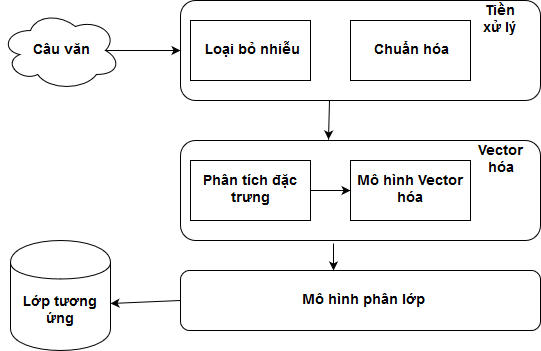
\includegraphics[scale=0.9]{image/Ml_Class_pipeline.png}
    \caption{Luồng xử lý cơ bản cho bài toán phân lớp bằng học máy}
    \label{fig:classication_pipeline}
\end{figure}
Lược đồ này có ba bước chính:
\begin{itemize}
    \item \textbf{Tiền xử lý:} Bước này được thực hiện để đạt được hai mục đích. Mục đích thứ nhất là loại bỏ các yếu tố gây nhiễu và làm tăng khả năng xử lý của bước tiếp theo. Mục đích thứ hai là chuẩn hóa để làm giảm số lượng các đặc trưng, hạn chế các trường hợp đặc trưng ngôn ngữ bị loại bỏ bởi vì định dạng của từ ngữ chú không phải dựa trên ngữ nghĩa của từ ngữ.
    \item \textbf{Vector hóa:} Mục đích của của bước này là số hóa ngôn ngữ. Không giống như con người có thể hiểu được và đánh giá được dữ liệu dựa trên ngữ nghĩa và tính chất của ngôn ngữ. Máy tính không có khả năng hiểu được dữ liệu biểu diễn dưới dạng ngôn ngữ mà chỉ có thể tính toán được dưới dạng số. Do đó, làm thế nào để có thể số hóa dữ liệu dạng văn bản nhưng đảm bảo giữ lại được đặc trưng về mặt ngữ nghĩa của dữ liệu, ít nhất là các đặc trưng nổi bật nhằm thực hiện được các tác vụ tương ứng là một thách thức rất lớn đòi hỏi sự phân tích và đánh giá một cách khéo léo các đặc trưng của dữ liệu. Sau khi thực hiện phân tích đặc trưng dữ liệu, các đặc trưng này sẽ được khai thác bằng các mô hình vector hóa phù hợp. Có hai mô hình cơ bản nhất nhưng đem lại hiểu quả lớn, bao gồm:
    \begin{itemize}
        \item \textbf{Bag of word ( BoW)} BoW là một thuật toán hỗ trợ xử lý ngôn ngữ tự nhiên giúp biểu diễn một văn bản dựa trên số lần xuất hiện của một từ trong văn bản. Đây là một cách biểu diễn rất tự nhiên và đơn giản nhưng lại đem lại hiệu quả rất tốt trong nhiều trường hợp mà phân loại văn bản là một ví dụ điển hình.
        
        Mô hình BoW được mô tả như hình \ref{fig:BoW}. Một mô hình BoW bao gồm một bộ từ điển, một hệ thống tiền xử lý ngôn ngữ (chuẩn hóa, loại bỏ từ, tách từ). Mô hình ghi nhớ toàn bộ bộ từ vựng có trong tập huấn luyện, hoặc một phần bộ từ điển. Mỗi từ sẽ được gán tương ứng với một vị trí nhất định. Một văn bản sẽ được biểu diễn bằng một vector với các phần tử ở những vị trí nhất định tương ứng là các số tự nhiên đại diện cho số lần xuất hiện của từ đó trong văn bản. Như vậy, BoW thể hiện được tần số xuất hiện của một từ bất kỳ trong văn bản mà dựa vào đó ta có thể đánh giá sự quan trọng của từ ngữ.
        \begin{figure}
            \centering
            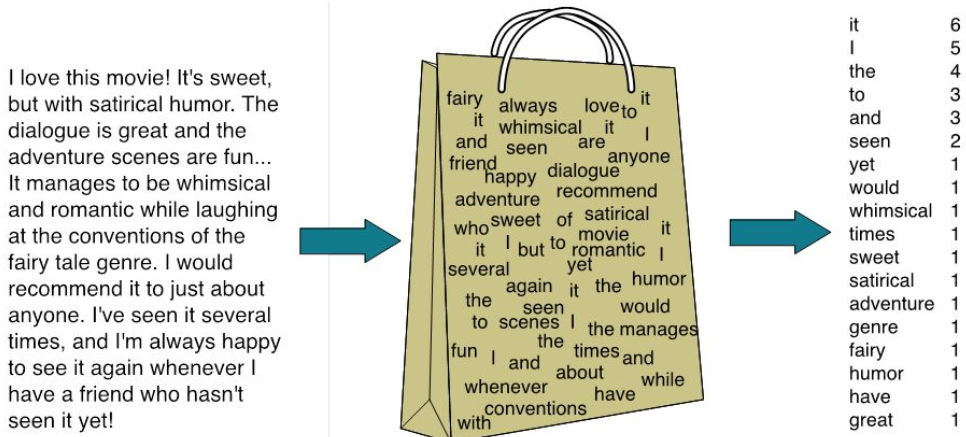
\includegraphics[scale=0.5]{image/BoG.PNG}
            \caption{Mô hình BoW}
            \label{fig:BoW}
        \end{figure}
        Đặc điểm của BoW là rất đơn giản. Dữ liệu được biểu diễn rời rạc nên phù hợp cho cả các mô hình xác suất. Tuy nhiên vì chỉ ghi nhận tần số xuất hiện của từ nên BoW gặp khó khăn trong việc đánh giá độ quan trọng của một từ ngữ, từ dó dẫn đến khuyết điểm là không phản ánh chính xác được tính chất của bộ dữ liệu.
        \item \textbf{Term frequency – Inverse document frequency (TFIDF)}
        Để khắc phục nhược điểm của BoW, mô hình TFIDF được đưa ra với cải tiến ở cách thức đánh giá về độ quan trọng của một từ.
        \begin{definition}
        TIDF của một từ là một con số thu được qua thống kê thể hiện mức độ quan trọng của từ này trong văn bản, mà bản thân văn bản đang xét nằm trong một tập hợp văn bản.
        \end{definition}
        TFIDF được tạo bởi hai phần: TF và IDF:
        \begin{itemize}
            \item \textbf{TF-term frequence} - tần số xuất hiện của một từ trong văn bản. Đại lượng này thể hiện khả năng một từ có thể đặc trưng cho một văn bản, theo nghĩa khi từ đó xuất hiện thì khả năng cao văn bản sẽ có nội dung tương tự.
            \begin{align*}
                tf(t, d)= \frac{f(t,d)}{\max \{f(w,d):w\in d\}}
            \end{align*}
            \begin{itemize}
                \item \textbf{$f(t,d)$}: số lần xuất hiện của từ $t$ trong văn bản $d$.
                \item \textbf{$\max \{ f(w,d) \}$}: Số lần xuất hiện nhiều nhất của một từ bất kỳ trong văn bản
            \end{itemize}
            \item \textbf{IDF- inverse document frequence} - Nghịch đảo tần số xuất hiện của một từ trong toàn bộ tập văn bản. Giá trị này dùng để giảm giá trị của những từ phổ biến, tức là xuất hiện nhiều ở các văn bản khác nhau, và do đó không thể hiện được đặc trưng của mỗi văn bản.
            \begin{align*}
                idf(t, D)= \log \frac{|D|}{|\{d \in D: t \in d \}|}
            \end{align*}
            \begin{itemize}
                \item $|D|$: Tổng số văn bản trong $D$
                \item $|\{d \in D: t\in d\}|$: Số văn bản chứa từ $t$ nhất định. Nếu từ $t$ không xuất hiện trong bất kỳ văn bản nào trong tập mẫu thì mẫu số sẽ bằng 0, do đó mấu số thương được thay thế bằng $1+|\{d \in D: t\in d\}|$.
            \end{itemize}
            \item $tfidf(t, d, D)= tf (t,d) \times idf(t,D)$
            
        \end{itemize}
    \end{itemize}
    \item \textbf{Mô hình phân lớp bằng học máy:} Các mô hình phân lớp hiệu quả cho việc phân loại dữ liệu là văn bản bao gồm các mô hình Bayes, mô hình máy vector hỗ trợ (SVM) và hô hình mạng neuron phân lớp (MLP). Mô hình Bayes áp dụng rất tốt cho các bài toán có tập dữ liệu nhỏ và các đặc trưng rõ ràng. Mô hình máy vector hỗ trợ có kết quả tổng quát hơn nhưng đòi hỏi tập dữ liệu huấn luyện lớn hơn. Còn đối với mô hình mạng neuron phân lớp, đây là một mô hình đem lại kết quả khá tốt kể cả với trường hợp đặc trưng dữ liệu không rõ ràng và tính nhập nhằng giữa dữ liệu trong các lớp lớn. Tuy nhiên vấn đề đối với mô hình mạng neuron là có thể xảy ra sự quá khớp (overfit) cho mô hình. Do đó, để làm việc tốt với mạng neuron phân lớp cần có các phương pháp huấn luyện phù hợp.\\
    Mô hình toán học của một MLP là ánh xạ (hàm) $y = f*(x, \theta)$ đi từ tập dữ liệu đầu vào đến tập dữ liệu đầu ra. Hàm này được cấu tạo từ nhiều hàm số đơn giản khác. Như vậy, bằng việc lựa chọn các hàm số cơ sở thích hợp và dữ liệu đầu vào, mô hình có thể xấp xỉ tham số $\theta$ và từ đó tạo ra các quy tắc $f(x)$ giúp máy tính có thể xác định được đầu ra.
    
    \begin{figure}[H]
        \begin{center}
            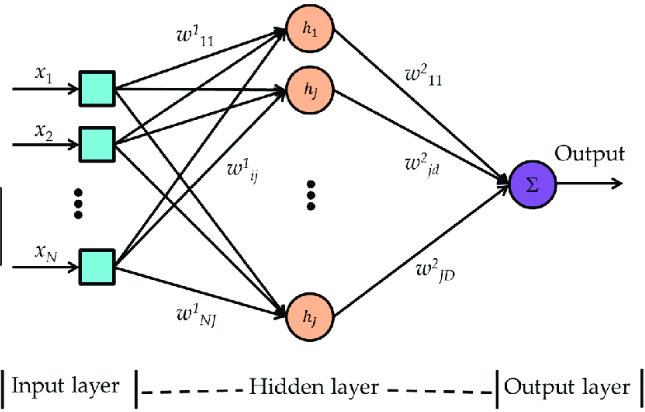
\includegraphics{image/MLP.PNG}
            \caption{Kiến trúc MLP}
            \label{fig:MLP} 
        \end{center}
    \end{figure}
    
    Thông thường, các tham số của mô hình trên được ước lượng thông qua việc tối ưu hàm chi phí $J(W, b, X, Y)$ bằng phương pháp hướng giảm nhanh nhất.
    Khi đó, ta cần tính hiệu quả các đạo hàm riêng $\frac{\partial J}{\partial W}$ và $\frac{\partial J}{\partial X}$.
    Một ví dụ về hàm chi phí là hàm trung bình của bình phương lỗi:
    $$J(W, B, X, Y) = \frac{1}{N} \sum_{n=1}^N \left \| y_n - a_n^l \right \|_2^2 $$
\end{itemize}
\subsection{Mô hình học sâu}
Việc áp dụng mô hình học sâu cho bài toán xử lý ngôn ngữ tự nhiên đã được áp dụng rất nhiều trong thời gian gần đây và đem lại kết quả ấn tượng. Có hai lý do cơ bản để các mô hình học sâu có thể đạt được những kết quả tốt là:
\begin{itemize}
    \item Có khả năng khai thác được các đặc trưng quan trọng nhất của ngôn ngữ.
    \item Có khả năng khai thác ngữ nghĩa theo tính chất tuần tự của dữ liệu.
\end{itemize}
Các kết quả tốt nhất hiện tại trong lĩnh vực xử lý ngôn ngữ tự nhiên đạt được bởi ba mô hình chính:
\begin{itemize}
    \item Mạng neuron tích chập - Convolution neural network
    \item Mạng bộ nhớ dài ngắn (LSTM)
    \item Cơ chế chú ý - Attention
\end{itemize}
Trong đó, mạng neuron tích chập thường được sử dụng ở mức độ ký tự, nhằm tìm kiếm các đặc trưng của chuỗi ký tự. Cơ chế attention lại tiếp cận theo hướng tìm các đặc trưng địa phương từ chuỗi ký tự, các đặc trưng này có thể là một từ hoặc một cụm từ. Tuy nhiên, cac mô hình hiện tại thường xây dựng bằng cách kết hợp CNN hoặc attention với mạng bộ nhớ dài ngắn - LSTM. Mạng LSTM có khả năng ghi nhớ các phụ thuộc xa của dữ liệu, là những đặc trưng rất quan trọng trong ngôn ngữ. Việc nhớ thông tin trong suốt thời gian dài là đặc tính mặc định của mạng, chứ ta không cần phải huấn luyện nó để có thể nhớ được. Tức là ngay nội tại của nó đã có thể ghi nhớ được mà không cần bất kì can thiệp nào. LSTM là một mạng neuron hồi quy - RNN, nhưng các mô-đun trong nó có cấu trúc khác với mạng RNN chuẩn. Thay vì chỉ có một tầng mạng neural, chúng có tới 4 tầng tương tác với nhau một cách rất đặc biệt theo sơ đồ sau.
\begin{figure}[h]
    \centering
    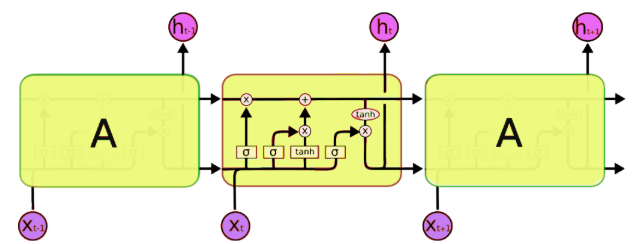
\includegraphics{image/LSTM.png}
    \caption{Mô hình LSTM}
    \label{fig:lstm}
\end{figure}
Chìa khóa của LSTM là trạng thái tế bào (cell state) - chính là đường chạy thông ngang phía trên của sơ đồ hình vẽ. Trạng thái tế bào là một dạng giống như băng truyền. Nó chạy xuyên suốt tất cả các mắt xích (các nút mạng) và chỉ tương tác tuyến tính đôi chút. Vì vậy mà các thông tin có thể dễ dàng truyền đi thông suốt mà không sợ bị thay đổi. LSTM có khả năng bỏ đi hoặc thêm vào các thông tin cần thiết cho trạng thái tế báo và được điều chỉnh cẩn thận bởi các nhóm được gọi là cổng là nơi sàng lọc thông tin đi qua nó.
    
Mặc dù kết quả của các mô hình học sâu rất tốt, nhưng nhược điểm của các mô hình này là đòi hỏi lượng dữ liệu huấn luyện rất lớn, mà hầu như là bất khả thi trong thực tế của các bài toán xử lý ngôn ngữ tự nhiên.


Như vậy, có thể thấy rằng hai phương pháp học sâu và học máy có những ưu và nhược điểm riêng biệt và tương phản nhau. Trong khi học máy đem lại kết quả tốt với tập dữ liệu nhỏ thì học sâu cần tập dữ liệu rất lớn để phát huy tính hiệu quả. Thay vào đó, kết quả của các mô hình học sâu mang tính tổng quát lớn hơn nhiều. Câu hỏi đặt ra là làm thế nào kết hợp được điểm mạnh của hai mô hình này. Để trả lời cho câu hỏi đó, phương pháp học chuyển tiếp ra đời và cho thấy sức mạnh của mình.

Phương pháp học chuyển tiếp đã đem lại kết quả rất tốt cho bài toán nhận diện thực thể tên và phân lớp ngôn ngữ. Cụ thể phương pháp sẽ được trình bày chương tiếp theo.

\chapter{Phương pháp học chuyển tiếp trong xử lý ngôn ngữ tự nhiên}
Học chuyển tiếp là một phương pháp học  trong tập trung vào việc khai thác các kiến thức thu được trong khi giải quyết một vấn đề và áp dụng nó vào một vấn đề khác nhưng có liên quan. Học chuyển tiếp là một bài toán liên quan đến vấn đề học đa tác vụ cũng như chuyển đổi ngữ cảnh, và bản thân học chuyển tiếp không chỉ là một lĩnh vực nghiên cứu của học sâu. Có hai phương pháp tiếp cận chính của học chuyển tiếp:
\begin{itemize}
    \item Phương pháp tiếp cận dựa trên phát triển mô hình:
    \begin{itemize}
        \item Lựa chọn tác vụ gốc: Tác vụ gốc được chọn là một tác vụ với lượng dữ liệu phong phú trong đó có một số mối quan hệ trong dữ liệu đầu vào, dữ liệu đầu ra và / hoặc các khái niệm đã học trong quá trình ánh xạ từ dữ liệu đầu vào sang đầu ra.
        \item Xây dựng mô hình: Xây dựng mô hình hiệu quả cho tác vụ gốc.
        \item Tái sử dụng mô hình: Mô hình được huấn luyện ở tác vụ gốc được sử dụng ở tác vụ đích, điều này có thể nâng cao hiệu quả của tất cả các thành phần của mô hình.
        \item Tinh chỉnh mô hình: Mô hình có thể phải điều chỉnh cho phù hợp với tác vụ đích.
    \end{itemize}
    \item Phương pháp tiếp cận dựa trên mô hình tiền huấn luyện:
    \begin{itemize}
        \item Lựa chọn mô hình gốc: Một mô hình gốc được đào tạo trước được chọn lựa từ các mô hình có sẵn. Nhiều nghiên cứu đã đưa ra các mô hình trên các bộ dữ liệu lớn và đầy thách thức có thể được đưa vào nhóm các mô hình tiềm năng để được lựa chọn.
        \item Tái sử dụng mô hình: Mô hình được huấn luyện ở tác vụ gốc được sử dụng ở tác vụ đích, điều này có thể nâng cao hiệu quả của tất cả các thành phần của mô hình.
        \item Tinh chỉnh mô hình: Mô hình có thể phải điều chỉnh cho phù hợp với tác vụ đích.
    \end{itemize}
\end{itemize}
Trong khuôn khổ luận văn này, em đã sử dụng phương pháp tiếp cận thứ hai bởi tính ưu việt và sự đa dạng của các kết quả đã đạt được trong phương pháp tiếp cận này những năm vừa qua trên thế giới.

Hai mô hình tiền huấn luyện được lựa chọn là BERT và Flair. Phần sau đây sẽ trình bày chi tiết về hai mô hình BERT và FLair. Trong đó Flair là mô hình biểu diễn ngôn ngữ dựa trên ngữ cảnh bằng việc mô hình hóa từ ngữ và ngữ cảnh là chuỗi tuần tự các ký tự. Flair được xây dựng dựa trên kiến trúc mạng mạng LSTM. FLair đem lại các kết quả ấn tượng cho các tác vụ xử lý gãn nhãn tuần tự theo chuỗi. BERT là mô hình biểu diễn hai chiều cho ngôn ngữ: \textbf{BERT:} Pre-training of Deep Bidirectional Transformers for Language Understanding. Mô hình này được xây dựng dựa trên kiến trúc Transformer với nền tảng là cơ chế attention. Các kết quả mới nhất cho thấy những kết quả ấn tượng của mô hình này với các bộ dữ liệu quan trọng của xử lý ngôn ngữ tự nhiên. Trước hết là những kiến thức nền tảng về cơ chế attention.

\section{Cơ chế attention}
\subsection{Tổng quan về cơ chế attention}
Cơ chế attention được sinh ra dựa trên nhu cầu cho việc ghi nhớ những câu dài, một trong những vấn đề cơ bản của máy dịch. Attention cho phép mô hình tập trung vào một hoặc một vài ngữ cảnh địa phương trong câu, đó cũng là nguồn gốc của tên gọi attention. Mục tiêu của attention là tính toán trạng thái tiếp theo của mô hình khi giải mã bằng cách tính toán trọng số dựa trên trạng thái của bộ mã hóa kết hợp với trạng thái phía trước của bộ giải mã. Các khái niệm mã hóa - giải mã là các khái niệm cơ bản được sử dụng trong máy dịch. Theo đó, bộ mã hóa cho phép mã hóa một chuỗi thành một vector, trong khi bộ giải mã thực hiện việc giải mã bộ vector đó thành chuỗi tương ứng.

Cơ chế attention ban đầu được đề xuất để giải quyết bài toán sequence-to-sequence thông thường bằng cơ chế mã hóa - giải mã. Attention được đưa vào để chỉnh sửa trọng số của vector trong phiên giải mã, giúp mô hình tập trung vào những thành phần quan trọng trong chuỗi thay vì toàn bộ chuỗi.
\begin{figure}
    \centering
    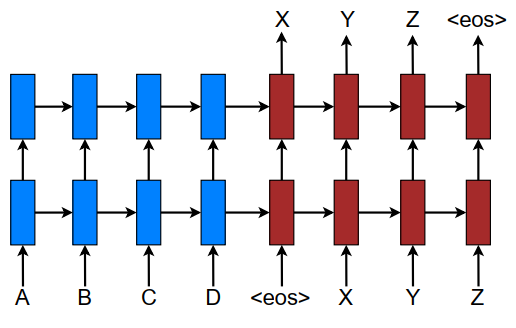
\includegraphics{image/luong_et_al.PNG}
    \caption{Mô hình sequence-to-sequence thông thường}
    \label{fig:luong_attention}
\end{figure}
Mô tả toán học của mô hình này như sau:
\begin{itemize}
    \item Encode:
\begin{align}
    h_{t}= f(x_{t}, h_{t-1})\\
    c= q(\{h_{1},...,h_{T_{x}}\})
\end{align}
    \item Decode:
\begin{align}
    p(\textbf{y})= \prod_{t=1}^{T} p(y_{t}|\{y_{1},..., y_{t-1}\}, c)\\
    p(y_{t}|\{y_{1},..., y_{t-1}\}, c)= g(y_{t-1}, s_{t}, c)
\end{align}
\end{itemize}
Mô hình attention đầu tiên được đề xuất bởi Bahdanau et. al. vào năm 2005 được gọi là soft-attention hay attention mềm. Mô hình toán học của phiên bản attention này được thể hiện như sau:
\begin{itemize}
    \item Hàm phân phỗi xác suất của bước giải mã: $p(y_{I}|\{y_{1},..., y_{i-1}\}, \textbf{x})=  g(y_{i-1}, s_{i}, c_{i})$
     với $s_{i}= f(s_{i-1}, y_{i-1}, c_{i})$
     \item Đưa ra một vector điều kiện $c_{i}$ tương ứng với từng thành phần của chuỗi $y_{i}$
     \item 
     \begin{align}
         c_{i}= \sum_{j=1}^{T_{x}}\alpha_{ij}h_{j}\\
         \alpha_{ij}= \frac{\exp (e_{ij}}{\sum_{k=1}^{T_{x}}\exp(e_{ik})}\\
         e_{ij}= a(s_{i-1}, h_{j})
     \end{align}
     Phương trình cuối cùng là một mô hình căn chỉnh trọng số mô tả sự tương ứng giữa giá trị đầu vào xung quanh vị trí $j$ và giá trị đầu ra tại vị trí $i$.
\end{itemize}
\begin{figure}
    \centering
    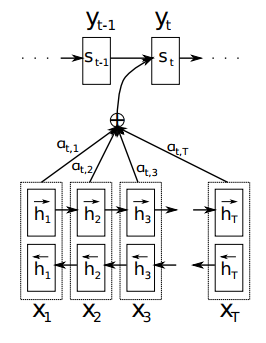
\includegraphics{image/bahaunau.PNG}
    \caption{Soft attention}
    \label{fig:bahaunau_att}
\end{figure}

\subsection{Các biến thể của attention}
Nhận thấy sự hiệu quả của mô hình attention, rất nhiều biến thể của attention được đưa ra cho nhiều mục đích khác nhau:
\begin{itemize}
    \item Hard attention:
    \begin{itemize}
    \item Xem xét attention như là các biến ẩn của mô hình
    \item Đưa vào một phân phối xác suất rời rạc được tham số hóa bởi  $\{\alpha\}$, và xem xét $c_{t}$ như một biến ngẫu nhiên. Phân phối xác suất được định nghĩa bởi: $p(s_{t, i}=1|s_{j<t}, \textbf{a})= \alpha_{t, i}$
    \item 
    \begin{align}
        c_{t}= \sum_{i}s_{t,i} x_{i}\\
        s_{t,i} \sim Multinoulli_{L}(\{\alpha\})
    \end{align}
    với $L$ là hàm mất mát $L_{s}= log(p(\textbf{y|a}))$
\end{itemize}
    \item Global attention: 
    Ý tưởng của mô hình attentional toàn cục là xem xét tất cả các trạng thái ẩn của bước mã hóa khi tính toán vector ngữ cảnh $c_{t}$
    \begin{figure}
    \centering
    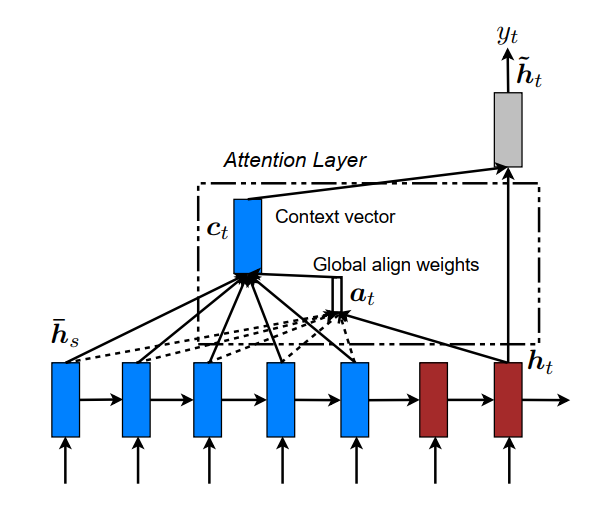
\includegraphics[scale=0.8]{image/global.PNG}
    \caption{Global attention }
    \label{fig:global_attention}
\end{figure}

\begin{itemize}
    \item \begin{align}
    \textbf{a}_{t}= \frac{\exp (score(\textbf{h}_{t},\overline{\textbf{h}}_{t} ))}{\sum_{s'}\exp (score(\textbf{h}_{t},\overline{\textbf{h}}_{s'} ))}
\end{align}
với:
\begin{itemize}
    \item $\textbf{h}_{s}$: trạng thái ẩn nguồn
    \item $\textbf{h}_{t}$: trạng thái ẩn đích
\end{itemize}
\item Global attention: content-based function
Có ba dạng chính:
\begin{itemize}
    \item Hàm nhân: $\textbf{h}_{t}^{T}\overline{\textbf{h}_{s}}$
    \item Hàm tổng quát: $\textbf{h}_{t}^{T}\textbf{W}_{a}\overline{\textbf{h}_{s}}$
    \item Hàm nối : $\textbf{v}_{a}^{T}tanh(\textbf{W}_{a}[h_{t}; \overline{h_{s}}])$
\end{itemize}
\begin{itemize}
    \item Tinh thần của global attention tương tự với Bahdanau et al. (2015)
    \item Global attention: $\textbf{h}_{t}\rightarrow \textbf{a}_{t} \rightarrow \textbf{c}_{t} \rightarrow \overline{\textbf{h}}_{t}$
    \item Soft attention: $\textbf{h}_{t-1}\rightarrow \textbf{a}_{t} \rightarrow \textbf{c}_{t} \rightarrow \textbf{h}_{t}$
\end{itemize}
\end{itemize}
\end{itemize}




\subsection{Seft attention}

Một cách tổng quát, ta có thể coi trạng thái phái trước của bộ giải mã là một vector truy vấn - query vector, trạng thái ẩn của bộ mã hóa là khóa - key và giá trị - value vector. Kết quả của attention là giá trị trung bình có trọng số của các vector giá trị, trong đó hệ số được tính toán dựa trên hàm tương thích giữa query và key. Chú ý rằng key và value  có thể là các bộ vector khác nhau.

Self-attentioon là quy trình áp dụng cơ chế attention được mô tả ở phần trên vào tất cả các vị trí của chuỗi đầu vào. Điều này được thực hiện bằng cách tạo ra bộ ba vector (query, key, value) cho tất cả các vị trí của chuỗi, sau đó áp dụng cơ chế attention cho mỗi vị trí $x_{i}$. Các vector key và query ở vị trí $x_{i}$ được sử dụng cho tất cả các vị trí khác. Đối với mỗi chuỗi đầu vào $X=(x_{1}, x_{2},...., x_{n})$ ta có chuỗi đầu ra tương ứng $Y=(y_{1}, y_{2},..., y)$ trong đó mỗi $y_{i}$ kết hợp thông tin của mỗi $x_{i}$ cũng như thông tin về cách thức $x_{i}$ liên quan đến các vị trí khác trong $X$. Bộ vector (query, key, value) có thể được tạo ra bằng cách sử dụng phép chiếu tuyền tính hoặc sử dụng mạng truyền thẳng.

Với một giá trị query $q$, các vector value $(v_{1}, v_{2},...,v_{n})$ và các vector key $(k_{1}, k_{2}, .. , k_{n})$, một giá trị đầu ra $z$ được tính toán dựa theo phương trình:
\begin{align}
    z= \sum_{j=1}^{n}\alpha_{j}(v_{j})\\
    \alpha_{j}=\frac{\exp{f(k_{j}, q}}{\sum_{i=1}^{n}\exp{f(k_{i}, q)}}
\end{align}
với $\alpha_{j}$ được tính toán bằng hàm softmax và $f(k_{i},q)$ là đặc trưng cho sự tương thích giữa $k_{i}$ và $q$.

Hàm tương thích thường được sử dụng là dot-product function:
\begin{align}
    f(k,q)= (k)(q)^{T}
\end{align}
hoặc hàm nhân scaled dot-product function:
\begin{align}
    f(k,q)=\frac{(k)(q)^{T}}{\sqrt{d_{k}}} 
\end{align}
trong đó $d_{k}$ là số chiều của key vectors. Việc giảm giá trị của hàm $f$ nhằm mục đích tăng sự ổn định khi chiều của các vector key, value cũng như query tăng lên.

Việc tính toán này có thể được thực hiện một các song song cho toàn bộ chuỗi đầu vào bằng cách nhóm các vector query, key, value tương ứng thành các ma trận $Q, K, V$, khi đó:
\begin{align}
    Attention(Q, K, V)= softmax(\frac{QK^{T}}{\sqrt{d_{k}}}V
\end{align}

\subsection{Multi-head attention}
Thay vì chỉ sự dụng cơ chế self-attention một lần cho $(Q, K, V)$ với số chiều $d_{model}$, cơ chế multi-head attention được đưa ra bằng cách tính toán attention $h$  lần với số chiều tương ứng $d_{model}/h$. Với mỗi head, bộ ma trận $(Q, K, V)$ được chiều riêng biệt lên không gian $d_{model}/h$ chiều và tính toán self-attention. Kết quả của mỗi head sau đó được nối lại và áp dụng một phép chiếu tuyền tính để đưa về không gian có số chiều tương ứng với bộ $(Q, K, V)$ ban đầu.

Mô hình tính toán được mô tả như sau:
\begin{align}
    MultiHead(Q,K,V)&= Concat(head_{1},...,head{n})W^{0} \\    
    head_{i}&= Attention(QW_{i}^{Q}, KW_{i}^{K}, VW_{i}^{V})
\end{align}
với $W_{i}^{Q}\in \mathbb{R}^{d_{model}\times d_{k}}$, $W_{i}^{K}\in \mathbb{R}^{d_{model}\times d_{k}}$,\\ $W_{i}^{V}\in \mathbb{R}^{d_{model}\times d_{v}}$ và $W^{0}\in \mathbb{R}^{hd_{v}\times d_{model}}$

\section{Mô hình Transformer}
Transformer là một mô hình không sử dụng hồi quy và dựa hoàn toàn trên cơ chế attention để thể hiện sự phụ thuộc toàn cục giữa đầu vào và đầu ra dữ liệu.
\subsection{Kiến trúc mô hình}
Transformer có kiến trúc mã hóa - giải mã. Ở đây, bộ mã hóa ánh xạ một chuỗi ký tựu đầu vào $(x_{1}, x_{2},...,x_{n})$ thành một chuỗi 
biểu diễn liên tục $\textbf{z}=(z_{1}, z_{2},...,z_{n})$. Sau khi có $\textbf{z}$, bộ giải mã thực hiện sinh ra chuỗi $(y_{1}, y_{2},..., y_{n})$ tương ứng.
\begin{figure}
    \centering
    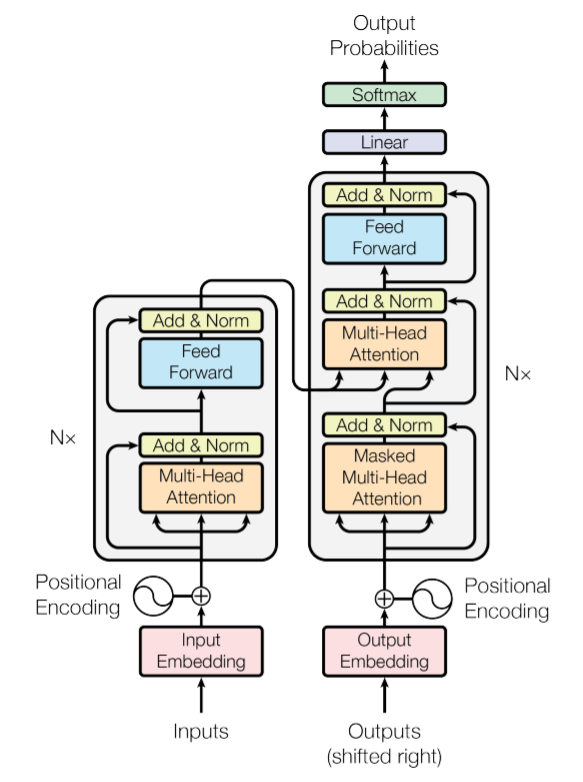
\includegraphics{image/transformer.PNG}
    \caption{Mô hình Transformer}
    \label{fig:Transformer}
\end{figure}
\subsection{Lớp mã hóa và giải mã}
\subsubsection{Lớp mã hóa}
Lớp mã hóa được hợp thành bởi $6$ khối nhỏ hơn giống y hệt nhau. Mỗi khối có hai lớp con, trong đó  lớp đầu tiên là một multi-head self-attention như đã mô tả ở trên. Lớp thứ hai là một mạng neuron đầy đủ truyền thẳng.  Lớp mã hóa sử dụng các kết nối dư xung quanh mỗi lớp con được đi theo bởi một lớp chuẩn hóa, tức là đầu ra của mỗi lớp con là một $LayerNorm(x+Sublayer(x))$, với $Sublayer(x)$ là hàm được thực hiện bằng chính bản thân layer con đó. Đầu ra này là một vector có số chiều là $d_{model}=512$.
\subsubsection{Lớp giải mã}
Lớp giải mã cũng được tạo bởi $6$ khối giống hệt nhau. Tuy nhiên ở lớp giải mã, ngoài hai lớp con tương tự như các khối của lớp mã hóa, lớp giải mã được chèn thêm một lớp con thứ ba để thực hiện multi-head attention trên đầu ra của lớp mã hóa. Tương tự như lớp mã hóa, ta sử dụng các kết nối dư xung quanh mỗi lớp con được đi theo bởi một lớp chuẩn hóa. Ở lớp giải mã này, lớp con self-attention cũng được chỉnh sửa để tránh tập trung vào các vị trí tiếp theo trong chuỗi. Điều này được thực hiện bỏi một lớp mặt nạ, kết hợp với giá trị nhúng đầu ra được bù bởi một giá trị vị trí để đảm bảo rằng giá trị dự đoán cho vị trí $i$ chỉ có thể phụ thuộc vào các giá trị đầu ra đã biết trước của các vị trí nhỏ hơn $i$.

\subsection{Áp dụng attention vào Transformer}
Mô hình Transformer sử dụng multi-head attention theo ba cách khác nhau:
\begin{itemize}
    \item Trong liên kết giữa lớp mã hóa và giải mã, vector truy vấn đưuọc lấy từ lớp giải mã phía trước trong khi vector khóa và vector giá trị được lấy từ giá trị đầu ra của lớp mã hóa. Điều này cho phép mọi vị trí của lớp mã hóa sẽ được tập trung từ tất cả các vị trí của chuỗi giá trị đầu vào, tức là thực thi tư tưởng truyền thống của mô hình sequence-to-sequence.
    \item Lớp mã hóa sử dụng các lớp self-attention với cả ba vector khóa, giá trị và truy vấn đều được lấy từ giá trị đầu ra của khối phía trước trong lớp mã hóa. Mỗi vị trí trong ớp mã hóa có thể chú ý đế tất cả các vị trí của lớp phía trước.
    \item Tương tự, các lớp self-attention trong lớp giải mã cho phép mỗi vị trí tập trung vào tất cả vị trí của khối phía trước.Tuy nhiên ta cần phải tránh việc ảnh hưởng trái luồng thông tin trong lớp giải mã để đảm bảo đặt tính tự hồi quy bằng cách đánh dấu tất cả các giá trị đầu vào lớp softmax tương ứng với các kết nối không hợp lệ giá trị $-\infty$.
\end{itemize}


\section{BERT-Mô hình biểu diễn hai chiều tiền huấn luyện}
Xuất hiện cuối năm 2018, BERT dược coi là một trong những mô hình tốt nhất trong lĩnh vực xử lý ngôn ngữ tự nhiên. BERT được đưa ra là giải pháp hiệu quả nhất để đối diện với thách thức về sự thiếu hụt dữ liệu đào tạo trong lĩnh vực xử lý ngôn ngữ tự nhiên. Bằng cách học tập mối quan hệ ngữ nghĩa giữa các từ ngữ và các câu trong một tập dữ liệu rất lớn nhờ các tác vụ học không giám sát, mô hình có thể học được các kiến thức tổng quan trong nghôn ngữ và là nền tảng để áp dụng vào các tác vụ cụ thể.
\subsection{Kiến trúc BERT}
Mô hình BERT là mô hình mã hóa sử dụng nhiều lớp Transformer mã hóa hai chiều, trong đó các lớp Transformer được sử dụng hoàn toàn tương tự như mô hình được đề xuất và thực thi gốc của Vasawani et al. (2017). Kiến trúc của Transformer được nói rất kỹ ở phần trên và việc thực thi kiến kiến trúc này trong BERT là hoàn toàn giống với cách thức triển khai gốc đó.

Mô hình BERT định nghĩa số lượng lớp (khối Transformer) là $L$, kích thức lớp ẩn là $H$ và số lượng head của self-attention là $A$. In tất cả các trường hợp, BERT đặt kích thước của lớp truyền thẳng là $4H$, tức là 3072 với $H= 768$ và 4096 với $H=1024$.

BERT tập trung vào hai mô hình sau:
\begin{itemize}
    \item \textbf{$BERT_{BASE}$:} $L=12, H=768, A=12$  với tổng cộng 110 triệu tham số
    \item \textbf{$BERT_{LARGE}$: } $L=24,H=1024,A=16$  với tổng cộng 340 triệu tham số
\end{itemize}

\subsection{Biểu diễn dữ liệu đầu vào}
Cách thức biểu diễn dữ liệu đầu vào của BERT cho phép biểu diễn đồng thời một câu hoặc một cặp câu trong một chuỗi biểu diễn. Với một từ cho trước, biểu diễn của từ đó được tạo bởi tổng hợp của các gái trị nhúng tương ứng với từ ngữ, đoạn cũng như vị trí. Cụ thể hơn:
\begin{figure}
    \centering
    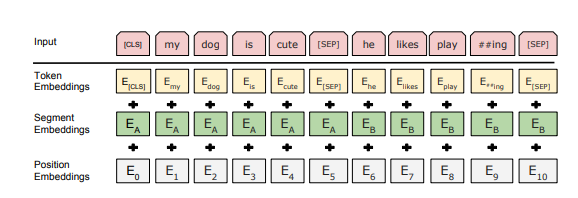
\includegraphics{image/Bert_input.png}
    \caption{Biểu diễn dữ liệu đầu vào của BERT}
    \label{fig:input_bert}
\end{figure}
\begin{itemize}
    \item BERT sử dụng WordPiece (Wu et al. 2016) để tách các câu thành các từ nhỏ với bộ từ điển bao gòm 30000 từ.
    \item Lớp nhúng vị trí được sử dụng với độ dài tối đa 512
    \item Ký tự đầu tiên của mọi chuỗi luôn luôn là ký tự đặc biệt ([CLS]) đại diện cho cả câu và sử dụng cho tác vụ phân lớp.
    \item Một cặp chuỗi được ghép lại với nhau vào cùng một chuỗi đơn, phân biệt bởi hai dấu hiệu:
    \begin{itemize}
        \item Dấu hiệu thứ nhất là sử dụng ký tự ngăn cách ([SEP])
        \item Dấu hiệu thứ hai là sự dụng giá trị nhúng câu $A$ đã được học cho chuỗi đầu tiên và giá trị nhúng $B$ cho chuỗi thứ hai. Đối với tác vụ chỉ sử dụng một câu đơn, BERT chỉ sử dụng duy nhất giá trị nhúng $A$.
    \end{itemize}
\end{itemize}
\subsubsection{Tác vụ tiền huấn luyện}
BERT được tiền huấn luyện bởi hai tác vụ học không có giám sát, đó là \textbf{Mô hình ngôn ngữ đánh dấu - Masked LM} và \textbf{Dự đoán câu tiếp theo - Next Sentence Prediction}
\subsubsection{Tác vụ 1: Masked LM}
Một cách trực quan, việc tin tưởng rằng một mô hình hai chiều mạnh hơn đáng kể so với các mô hình một chiều là có ý nghĩa. Tuy nhiên không may là các mô hình ngôn ngữ thông thường chỉ có thể được huấn luyện theo chiều từ trái sang phải hoặc từ phải sang trái, trong khi điều kiện hai chiều nên cho phép mỗi từ ngữ được xem xét trực tiếp chính bản thân từ ngữ đó trong nhiều lớp ngữ cảnh khác nhau.

Để có thể huấn luyện một biểu diễu sâu hai chiều cho ngôn ngữ, BERT sử dụng một cách tiếp cận trực tiếp đó là đánh dấu ngẫu nhiên một số lượng từ đầu vào vào sau đó thực hiện dự đoán những từ ngữ đã được đánh dấu này. Trong trường hợp này, vector hẩn cuối cùng tương ứng với các từ bị đánh dấu sẽ được truyền qua một lớp softmax trên toàn bộ bộ từ điển tương tự như các mô hình ngôn ngữ thông thường. BERT thực hiện đánh dấu ngẫu nhiên $15\%$ tất cả các từ ngữ trong WordPiece trong mỗi chuỗi đầu vào. Để tránh nhiễu, BERT thực hiện dự đoán các từ bị đánh dấu thay vì cấu trúc lại toàn bộ chuỗi đầu vào.

Cách tiếp cận này vẫn tồn tại hai nhược điểm sau khi nhận được  mô hình tiền huấn luyện theo hai chiều. Nhược điểm thứ nhất là BERT tạo ra sự không phù hợp giữa hai quá trình tiền huấn luyện và quá trình tinh chỉnh mô hình, tức là là ký tự [MASK] sẽ không bao giờ xuất hiện trong quá trình tinh chỉnh. Để giảm thiểu vấn đề này, BERT không luôn luôn đánh dấu ký tự bằng [MASK]. Thay vào đó:
\begin{itemize}
    \item Thay thế $80\%$ số lượng từ được chọn bằng [MASK]
    \item Thay thế $10\%$ số lượng từ được chọn bằng một từ bất kỳ khác
    \item Giữ nguyên $10\%$ số lượng từ được chọn  
\end{itemize}
Lớp Transformer mã hóa không biết trong tập hợp các từ được chọn, từ nào sẽ bị thay thế bằng những từ khác và từ nào sẽ được giữ nguyên, do đó mô hình sẽ học được phân phối của tất cả các từ. Thêm vào đó, bởi vì việc thay thế ngẫu nhiên chỉ xảy ra cho $1.5\%$ số lượng các từ nên có vẻ sẽ không ảnh hưởng đến tính phù hợp của việc thu nhận kiến thức cho mô hình ngôn ngữ.

Nhược điểm thứ hai của việc sử dụng MLM là chỉ có $15\%$ số lượng từ ngữ được dự đoán nên mô hình sẽ hội tụ chậm hơn rất nhiều so với mô hình tuần tự từ rái sang phải. 

\subsubsection{Tác vụ 2: Next Sentence Prediction}
Rất nhiều tác vụ thực tế được dựa trên kiến thức về mối liên hệ giữa hai câu văn, trong khi những kiến thức này không được thu nhận trực tiếp bởi mô hình ngôn ngữ. Để có thể huấn luyện mô hình có thể hiểu được mối quan hệ giữa các từ ngữ, BERT sử dụng tác vụ \textit{next sentence prediction} có thể được tạo ra một cách đơn giản bởi bất kỳ bộ dữ liệu đơn ngôn ngữ nào. Ví dụ:
\begin{itemize}
    \item Intput = \textit{[CLS] the man went to [MASK] store [SEP] he bought a gallon [MASK] milk [SEP]}
    \item Label = \textit{IsNext}
    \item Input = \textit{[CLS] the man [MASK] to the store [SEP] penguin [MASK] are flight \#\#less birds [SEP]}
    \item Label = \textit{NotNext}
\end{itemize}
Trong đó nhãn \textit{IsNext} thể hiện rằng đây là hai câu liên tiếp và nhãn \textit{NotNext} thể hiện rằng hai câu này không phải là hai câu liên tiếp nhau. 



\section{Flair}
Flair là một mô hình nhúng từ sử dụng ngữ cảnh hóa tại cấp độ ký tự với mục đích bao quát và kết hợp các thuộc tính tốt nhất của các mô hình nhúng từ ngữ hiện tại. Mô hình này có ba khả năng sau:
\begin{itemize}
    \item Được tiền huấn luyện trên một tập văn bản rất lớn bằng tác vụ học không giám sát
    \item Ghi nhận ý nghĩa của từ ngữ trong ngữ cảnh nhất định
    \item Mô hình hóa từ ngữ và ngữ cảnh dựa trên chuỗi ký tự, giúp kiểm soát được các từ ngữ hiếm và sai chính tả một cách tốt nhất
\end{itemize}
Kiến trúc nền tảng của Flair là mô hình mạng LSTM đã được nói đến ở chương 1.

\subsection{Tổng quan mô hình dự đoán chuỗi sử dụng Flair}
Mô hình dự đoán này sử dụng một mạng LSTM hai chiều  trên dữ liệu vào đã được xử lý bởi lớp nhúng. Kết quả của mạng LSTM hai chiều sau đó được truyền qua một mạng neuron với một lớp ẩn, để lấy kết quả tương ứng là vector xác suất $a_{i}$ tương ứng với từng lớp tương tự như các mô hình thông thường.
\begin{figure}[H]
    \centering
    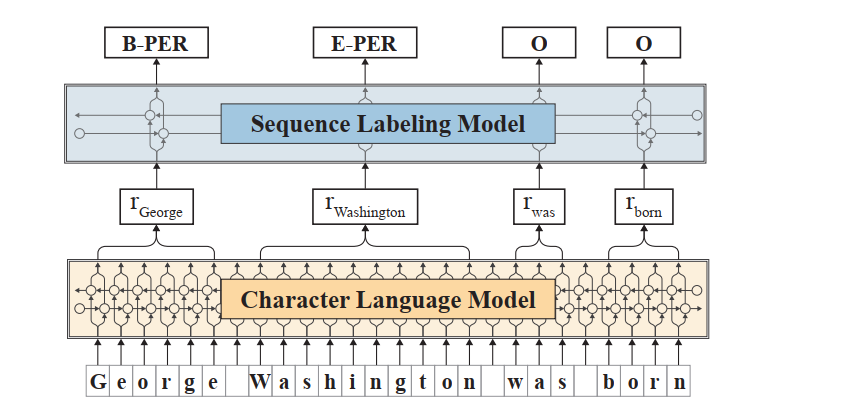
\includegraphics[scale=0.8]{image/flair_taging.PNG}
    \caption{Mô hình gán nhãn tuần tự}
    \label{fig:sequence_labeling}
\end{figure}
Sau đó vector xác suất kết quả của lớp dự đoán sử dụng BiLSTM sẽ tiếp tục được đừa vào mô hình CRF để đưa ra kết quả là chuỗi nhãn tương ứng với chuỗi dữ liệu ban đầu. Chiến thuật đưa ra cho lớp này là đánh giá điểm  số của một chuỗi dự đoán $y_{i:n}$ dựa trên hai thành phần. Thành phần thứ nhất là xác suất thu được từ kết quả của lớp dự đoán. Thành phần thứ hai là phân phối xác suất của hai chuỗi nhãn dán, ký hiệu là $T[i,j]$ tương ứng là xác suất cả một từ tố có nhãn $i$ được theo sau bởi một từ tố có nhãn $j$, và xác suất này được học bởi mô hình $CRF$. Cụ thể, điểm số của một chuỗi dự đoán được tính toán như sau:
\begin{align}
    s(y_{i:n})= \sum_{i=1}^{n} \textbf{a}_{i}[y_{i}] + \sum_{i=2}^{n}T[y_{i-1}, y_{i}]
\end{align}

\subsection{Lớp nhúng từ }
Lớp nhúng từ - Word embedding - là trọng tâm của Flair. như đã nói ở trên, lớp nhúng này tích hợp đầy đủ các đặc tính tốt của các mô hình nhúng thông thường, do đó gia tăng một cách hiệu quả độ chính xác của các mô hình dự đoán. Lớp nhúng từ bao gồm hai thành phần quan trọng nhất đó là lớp nhúng theo ngữ cảnh giúp Flair học được mối quan hệ ngữ nghĩa và biểu diễn từ dựa trên chuỗi ký tự. Thành phần thứ hai là mô hình xếp chồng các lớp nhúng, giúp khai thác sự hiệu quả đến từ các mô hình embedding khác.
\subsubsection{Lớp nhúng ngữ cảnh }
Lớp nhúng ngữ cảnh - Contextual string embeddings - với bản chất là một mạng LSTM, được huấn luyện bằng cách sử dụng mô hình ngôn ngữ tại cấp độ kí tự, và được huấn luyện để dự đoán kí tự tiếp theo của câu. Nghĩa là mô hình xem xét đến trạng thái ẩn của mỗi kí tự trong câu và sử dụng trạng thái ẩn này đại diện cho ký tự đó.
Mục tiêu của mô hình ngôn ngữ tầng kí tự là để ước lượng phân phối $P(x_{0:T} )$ thông qua chuỗi kí tự $(x_0,x_1,…,x_T )$ của ngôn ngữ xử dụng. Bằng việc huấn luyện mô hình ngôn ngữ, ta có thể xác định được $P(x_t |x_0,…,x_{t-1})$ để dự đoán phân phối của kí tự tiếp theo khi biết các kí tự trước hoặc sau của nó, tùy theo chiều xem xét của LSTM. Phân phối chung trên toàn bộ câu có thể được tách thành tích các phân phối có điều kiên trên các kí tự đã có:
\begin{align*}
    P(x_{0:T} )=\prod_{t=0}^T P(x_t |x_{0:t-1})
\end{align*}

Trong kiến trúc mạng LSTM, xác suất điều kiện $P(x_t |x_{0:t-1})$ được tính xấp xỉ thông qua đầu ra $h_t$
\begin{align*}
    P(x_t |x_{0:t-1}) \approx \prod_{t=0}^T P(x_t |h_t;\theta)
\end{align*}
\begin{figure}[H]
    \centering
    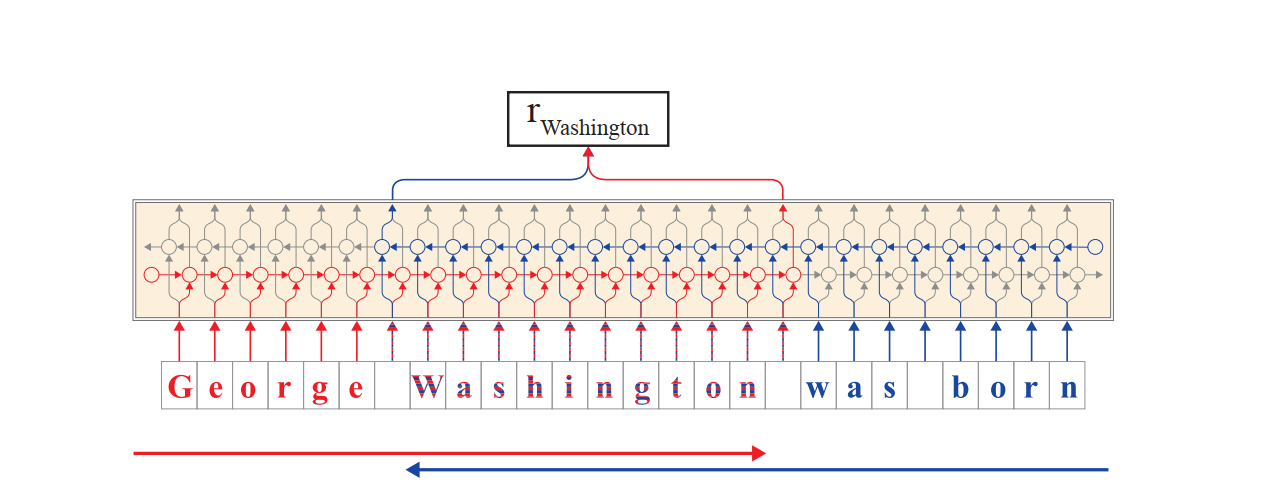
\includegraphics[scale=0.7]{image/flair_lm.PNG}
    \caption{Mô hình ngôn ngữ Flair}
    \label{fig:flair_lm}
\end{figure}
Để tạo đại diện cho một từ, ta sẽ sử dụng các mô hình xuôi (forward)  và ngược (backward) với kiến trúc giống nhau nhưng hướng dự đoán khác nhau (forward model dự đoán kí tự tiếp theo còn backward model dự đoán kí tự trước đó). Đối với forward model ta sẽ sử dụng đầu ra của hidden state sau khi truyền kí tự cuối cùng của từ qua model, còn backward model thì ta sẽ sử dụng đầu ra của hidden state sau khi truyền kí tự đầu tiên của từ qua model.

\subsubsection{Xếp chồng các lớp nhúng }
Việc xếp chồng các lớp nhúng -  Stack Embeddings - cho phép mô hình khai thác được ưu điểm của các mô hình nhúng khác nhau. Việc xếp chồng các lớp nhúng này đơn giản được thực hiện bằng cách ghép nối các vector nhúng lại với nhau tạo thành một vector nhúng duy nhất cho từ đang được xem xét.



\chapter{Hệ thống trích lọc và phân tích thông tin trong văn bản tài chính sử dụng học chuyển tiếp}

\section{Kiến trúc hệ thống}
Hệ thống sử dụng hai mô hình khác nhau, mô hình thứ nhất là mô hình nhận diện thực thể tên để trích lọc thông tin từ văn bản. Mô hình thứ hai là mô hình phân lớp câu văn để đánh giá tính chất của các câu văn tương ứng. 

\subsection{Mô hình nhận diện thực thể tên}
Mô hình nhận diện thực thể tên được sử dụng là mô hình gán nhãn chuỗi của Flair. Mô hình này đã được trình bày ở chương trước.
\subsubsection{Kích thước tập dữ liệu}
Tập dữ liệu bao gồm các câu văn chứa thông tin được chọn lựa ngẫu nhiên từ tập văn bản báo cáo tài chính và được gán nhãn bằng tay. Tập dữ liệu này gồm có:
\begin{itemize}
    \item Tập huấn luyện chiếm $80\%$ kích thước tập dữ liệu, gồm 92 câu văn
    \item Tập đánh giá chiếm $20\%$ kích thước tập dữ liệu
\end{itemize}
\subsubsection{Tiền huấn luyện}
Việc huấn luyện lại lớp nhúng ngữ cảnh một cách tổng quát tiêu tốn rất nhiều chi phí, do đó lớp nhúng ngữ cảnh được huấn luyện bằng một tập nhỏ hơn dữ liệu được lấy trực tiếp từ các văn bản tài chính. Hay nói cách khác, mô hình được tiền huấn luyện trong ngữ cảnh của văn bản tài chính, tuy rằng điều này không đem lại một mô hình ngôn ngữ tổng quát, nhưng những kiến thức nền tảng về mối quan hệ từ ngữ trong các văn bản tài chính đã được ghi nhận.

Ngoài ra, mô hình còn sử dụng những mô hình nhúng đã được huấn luyện từ trước như byte-pair embedding được huấn luyện trên 207 ngôn ngữ và BERT embedding được huấn luyện trên 104 ngôn ngữ. Do đó, các kiến thức tổng quát và nền tảng về ngôn ngữ phần nào đã được ghi nhận bởi các mô hình embedding khác.
\subsubsection{Phương pháp đánh giá}
Mô hình sử dụng độ đo $F1-score$ và $accuracy$ để đánh giá độ chính xác của mô hình. $F1-score$ và $accuracy$ có công thức sau đây:
\begin{align}
    F1= 2\frac{precision \times recall}{precision + recall}\\
    acc= \frac{\text{number of correct predictions}}{\text{Total numbers of prediction}}
\end{align}
$F1-score$ được đánh giá dựa trên độ chính xác hoàn toàn (exact match) của thực thể được dự đoán so với thực thể gốc.
\subsubsection{Kết quả}
Mô hình đem lại kết quả khá tốt. Bảng \ref{tab:ner} thể hiện chi tiết kết quả của mô hình.

\begin{table}

\begin{tabular}{ |p{1.7cm}||p{1.6cm}|p{1.8cm}|p{1.7cm}|p{1.5cm}|p{1.5cm}|p{1.7cm}|  }
 \hline
 \hline
 Class & address & birthdate & company & gender & person & position \\
 \hline
 Precision &0.9886 & 0.7273 & 0.9539 & 1.000 & 0.7170 & 0.7955\\
 Recall    &0.816 & 1.0000 & 0.7073 & 1.000 & 0.6441 & 0.6667\\
 accuracy & 0.8084 & 0.7273 & 0.6840 & 1.000 & 0.5135 & 0.5691\\
 F1-score &   0.8940  & 0.8421 & 0.8123 & 1.000 & 0.6786 & 0.7254\\
\hline
 \multicolumn{7}{|c|}{MICRO\_AVG: acc 0.685 - f1-score 0.8131}\\
 \hline
  \multicolumn{7}{|c|}{MICRO\_AVG: acc 0.717 - f1-score 0.8254}\\
  \hline
 \multicolumn{7}{|c|}{Time: 2h}\\
  \hline
 \multicolumn{7}{|c|}{GPU: Tesla V100 16 Gb Memory}   \\
 \hline
\end{tabular}
\caption{Kết quả mô hình NER}
\label{tab:ner}
\end{table}

\subsection{Mô hình phân lớp câu văn}
\subsubsection{Tổng quan mô hình}
Mô hình phân lớp câu văn sử dụng BERT. Trong mô hình phân lớp câu văn này, giá trị đầu ra duy nhất được sử dụng cho lớp giải mã chính là giá trị đầu ra tương ứng với ký tự đặc biệt [CLS] được nói đến ở chương trước. Thông tin về ký tự này đại diện cho toàn bộ nội dung của câu văn, do đó nó có ý nghĩa chủ chốt trong mô hình phân lớp.
\begin{figure}
    \centering
    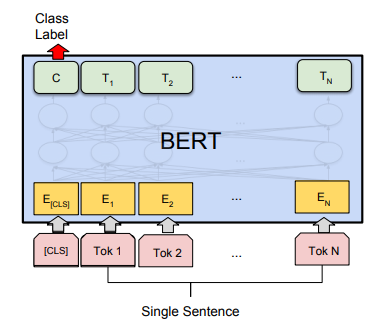
\includegraphics[scale=1.5]{image/bert_cls.png}
    \caption{Kiến trúc mô hình phân lớp câu văn}
    \label{fig:bert_cls}
\end{figure}
Gọi $c \in \mathbb{R}^{m}$ với $m$ là số chiều của vector đầu ra của lớp mã hóa tương ứng với ký tự [CLS], ta có xác suất của giá trị đầu ra của mô hình là:
\begin{align}
    P=softmax( Wc+b)
\end{align}
và nhãn tương ứng là $argmax(P)$
\subsubsection{Kích thước tập dữ liệu}
Tập dữ liệu bao gồm các câu văn được chọn lựa ngẫu nhiên từ tập văn bản báo cáo tài chính và được gán nhãn bằng tay. Tập dữ liệu này gồm có:
\begin{itemize}
    \item Tập huấn luyện chiếm $80\%$ kích thước tập dữ liệu, gồm 65 câu có nhãn Negative, 52 câu có nhãn Neutral và 153 câu có nhãn Positive
    \item Tập đánh giá chiếm $20\%$ kích thước tập dữ liệu, bao gồm 15 câu có nhãn Negatvie, 28 câu có nhãn Neutral và 35 câu có nhãn Positive
\end{itemize}

\subsubsection{Tiền huấn luyện và phương pháp đánh giá}
Mô hình được tiền huấn luyện bởi tập dữ liệu là tất cả dữ liệu dạng văn bản trên trang web Wikipedia và tập dữ liệu sách. Tập văn bản này bao gồm 104 ngôn ngữ khác nhau. Mô hình tiền huấn luyện có 110 triệu tham số.

Phương pháp đánh giá cho mô hình được sử dụng là $F1-score$ tương tự mô hình nhận diện thực thể tên.

\subsubsection{Kết quả}
Mô hình cho thấy kết quả phân loại các lớp Positive và Negative khá tốt. Lớp Neutral chưa được tốt nhưng do đặc trưng về ngôn ngữ dễ nhầm lẫn dữa Neutral và các lớp còn lại, do đó kết quả này là khá tốt. Bảng \ref{tab:cls} thể hiện chi tiết kết quả của mô hình.

\begin{table}[]
\begin{tabular}{ |p{3cm}||p{3cm}||p{3cm}||p{3cm}|  }
 \hline
 \hline
 Class &  Negative & Neutral & Positive \\
 \hline
 Precision & 0.79  & 0.64 & 0.74 \\
 Recall    & 0.73  & 0.39 & 0.91 \\
 F1-score  & 0.76  & 0.48 & 0.82 \\
 \hline
 micro avg & 0.74  & 0.74 & 0.74 \\
 micro avg & 0.72  & 0.68 & 0.69 \\
\hline
 \multicolumn{4}{|c|}{Time: 1h}\\
  \hline
 \multicolumn{4}{|c|}{GPU: Tesla V100 16 Gb Memory}   \\
 \hline
\end{tabular}
\caption{Kết quả phân lớp câu văn}
\label{tab:cls}
\end{table}
\section{Kết quả hệ thống}
Văn bản đầu vào có định dạng pdf. Hình \ref{fig:input_doc} là một văn bảo dữ liệu đầu vào hệ thống.\\
\begin{figure}
    \centering
    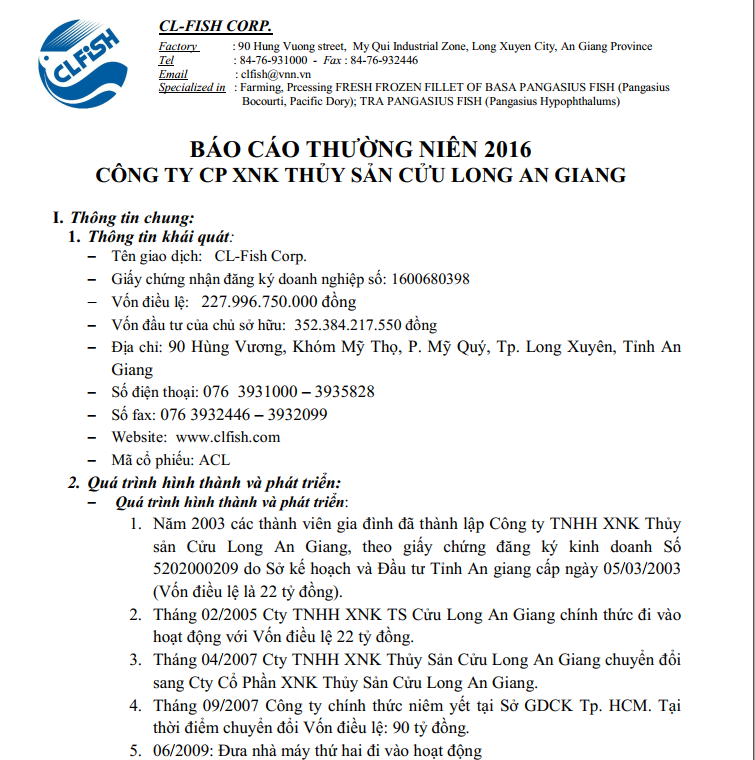
\includegraphics[scale= 0.5]{image/input_doc.PNG}
    \caption{Văn bản dữ liệu đầu vào}
    \label{fig:input_doc}
\end{figure}
Toàn bộ kết quả xử lý được hiển thị ở giao diện kết quả. Hình \ref{fig:output} là kết quả trả về cho văn bản phía trên.\\
\begin{figure}
    \centering
    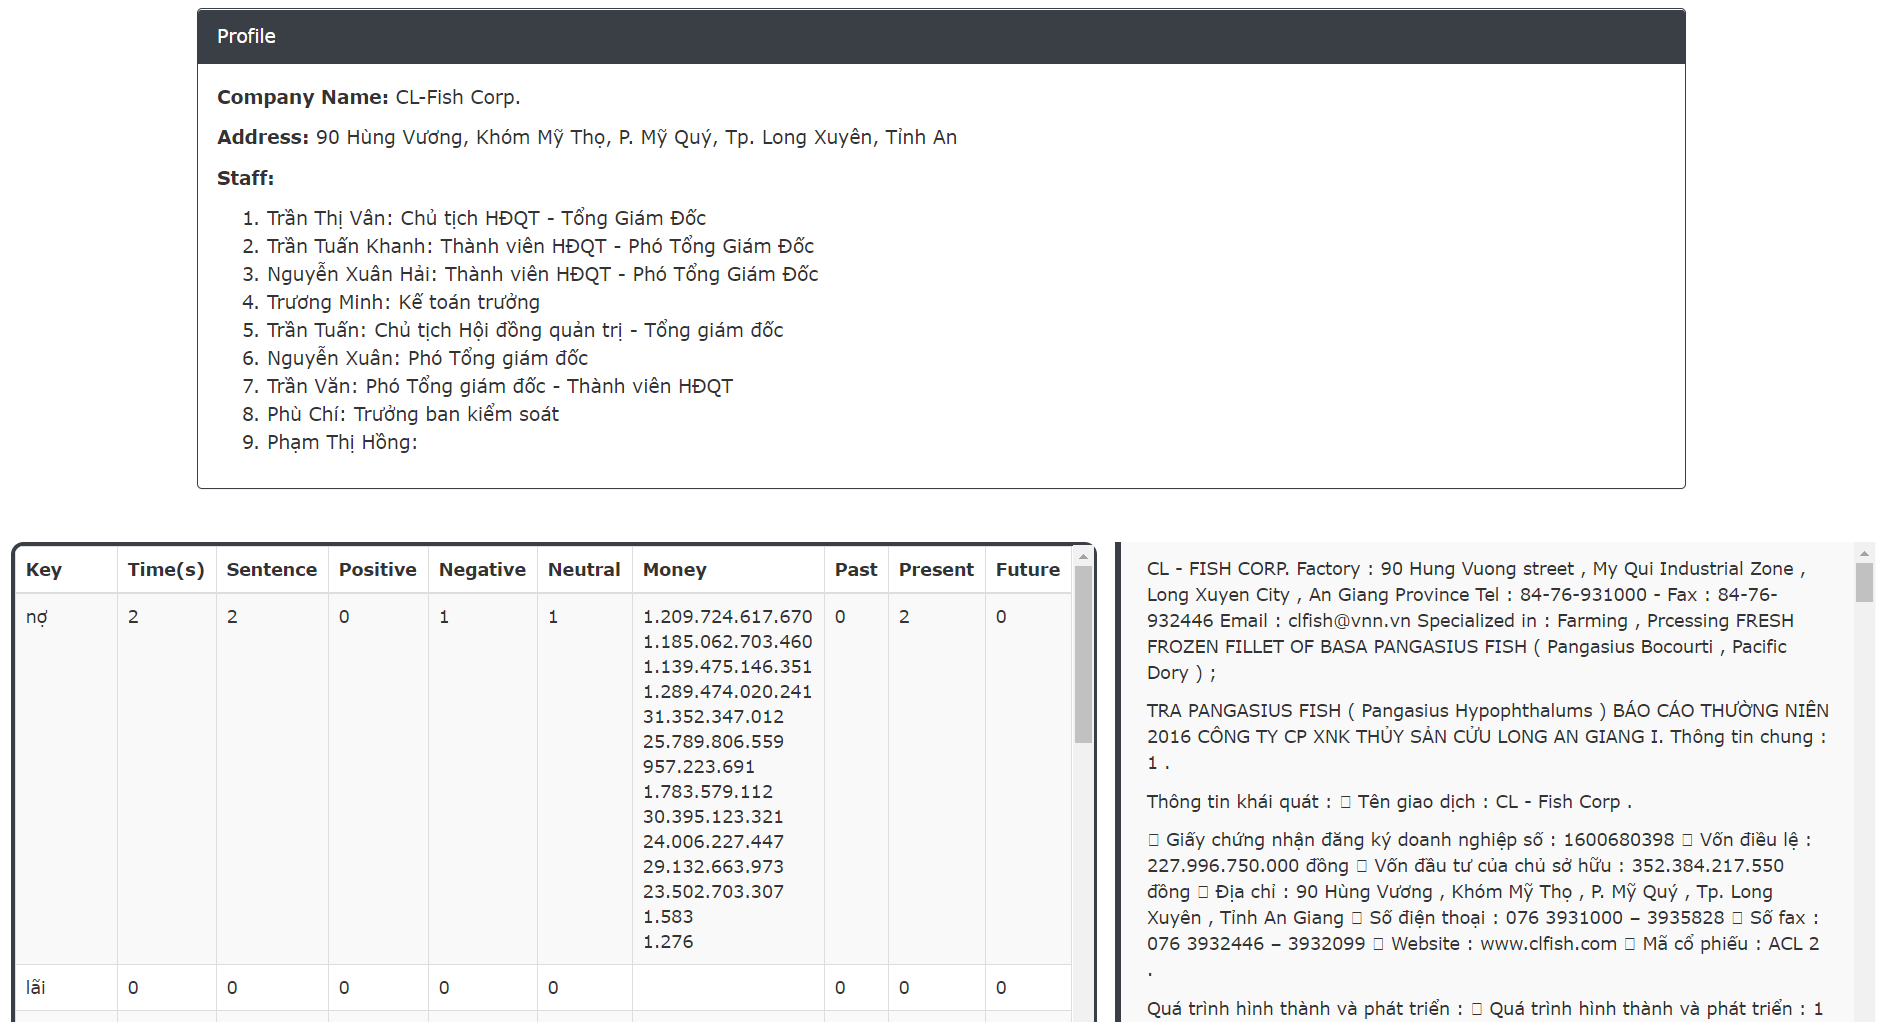
\includegraphics[scale= 0.4]{image/Output.PNG}
    \caption{Trang kết quả của hệ thống}
    \label{fig:output}
\end{figure}
Trang kết quả gồm 3 phần chính:
\begin{itemize}
    \item Kết quả đọc văn bản được mô tả ở \ref{fig:read}
    \item Kết quả trích xuất thông tin bao gồm thông tin về người, công ty được mô tả ở \ref{fig:extract} và các thông tin quan trọng nằm trong bảng ở \ref{fig:extract}
    \item Kết quả phân tích thông tin được thể hiện ở trong bảng được mô tả ở \ref{fig:analysis}
\end{itemize}
\begin{figure}
    \centering
    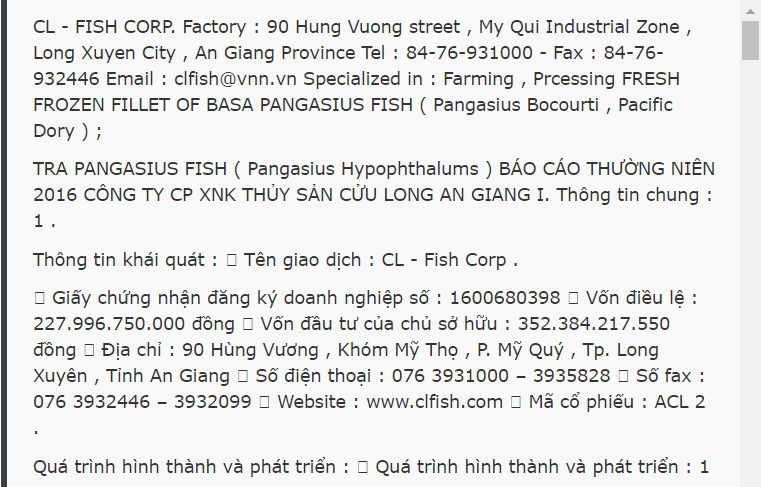
\includegraphics[scale= 0.7]{image/read.PNG}
    \caption{Kết quả đọc văn bản}
    \label{fig:read}
\end{figure}
\begin{figure}
    \centering
    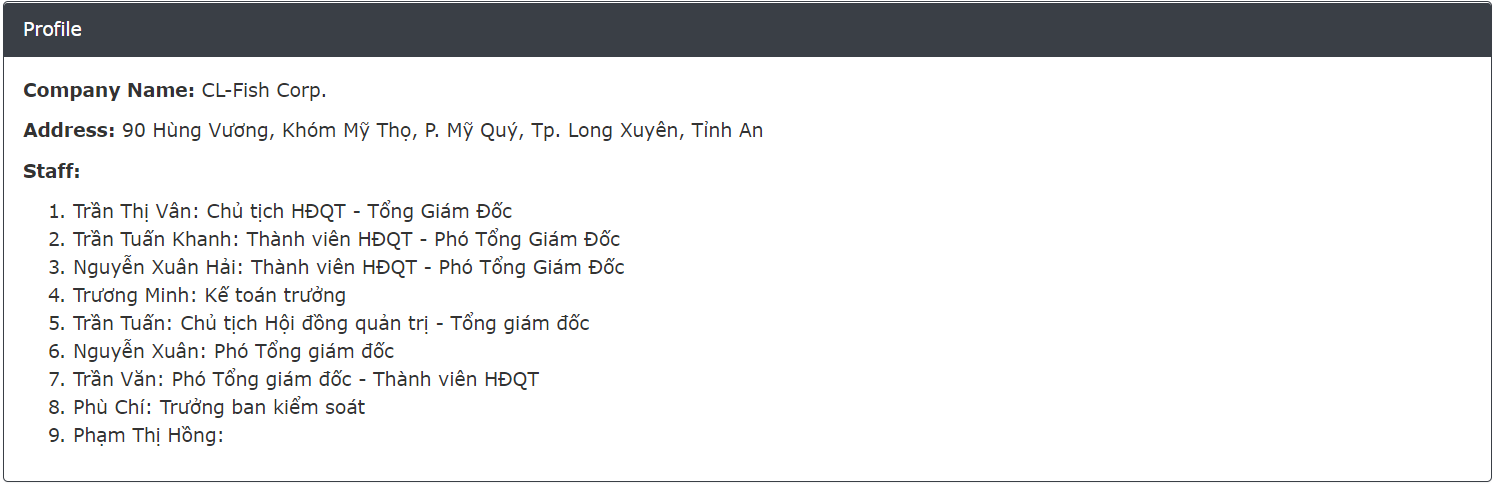
\includegraphics[scale= 0.4]{image/extract.PNG}
    \caption{Kết quả trích xuất thông tin tổng quan về công ty, cá nhân}
    \label{fig:extract}
\end{figure}
\begin{figure}
    \centering
    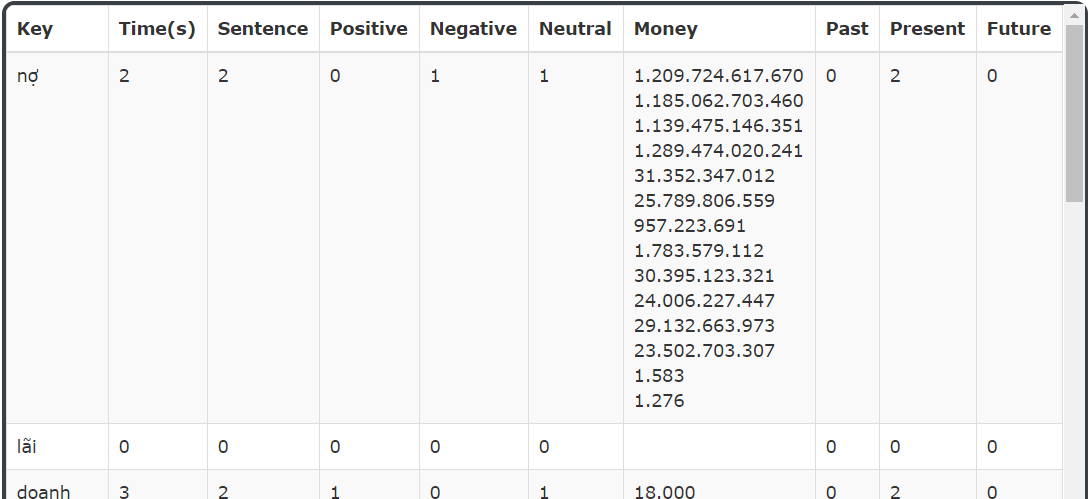
\includegraphics[scale= 0.6]{image/analysis.PNG}
    \caption{Kết quả phân tích và trích xuất các thông tin khác}
    \label{fig:analysis}
\end{figure}
\newpage
\section{Tổng kết}
Hệ thống trích xuất và phân tích thông tin tiếp cận và xử lý các văn bản dạng báo cáo tài chính. Đây là các văn bản phức tạp, đặc thù, đặt ra nhiều thách thức cho việc phân tích và đánh giá, tuy nhiên cũng đem lại nhiều lợi ích to lớn nếu được xử lý một cách hiệu quả.

Việc trích xuất và phân tích thông tin trong văn bản tài chính tập trung vào giải quyết hai bài toán: Nhận diện thực thể tên và Phân lớp câu văn. Đây là hai bài toán quan trọng trong lĩnh vực xử lý ngôn ngữ tự nhiên. Các phương pháp tiếp cận thông thường bao gồm học máy thống kê và học sâu. Các phương pháp này có những ưu điểm và nhược điểm riêng nhưng đều tỏ ra không hiệu quả trong hoàn cảnh tập dữ liệu nhỏ và tính đa dạng của dữ liệu lớn.

Học chuyển tiếp là một cách tiếp cận hiệu quả cho các bài toán có tập giữ liệu nhỏ bằng cách ghi nhận tri thức từ các bài toán lớn và tổng quát để áp dụng sang các bài toán cụ thể, từ đó giữ được tính tổng quát cao mặc dù tập dữ liệu huấn luyện không lớn. Hai mô hình học chuyển tiếp quan trọng và đem lại hiệu quả cao hiện tại là mô hình BERT với nền tảng là kiến trúc attention với nòng cốt là lớp mã hóa transformer và mô hình Flair xây dựng dựa trên mạng bộ nhớ dài ngắn LSTM , một biến thể của mạng neuron hồi quy RNN với khả năng mô hình hóa ngôn ngữ dưới dạng chuỗi các ký tự.

Các kết quả thực nghiệm cho thấy với tập dữ liệu nhỏ, đặc trưng dữ liệu rất đa dạng nhưng kết quả của hệ thống rất khả quan và có tính ứng dụng thực tiễn cao.
\newpage
\begin{thebibliography}{12}



\bibitem{FLAIR}
\textit{Alan Akbik, Duncan Blythe, Roland Vollgraf
} Contextual String Embeddings for Sequence Labeling
\url{https://www.aclweb.org/anthology/C18-1139}

\bibitem{soft_att}
\textit{Dzmitry Bahdanau, KyungHyun Cho, Yoshua Bengio} Neural machine translation by jontly learning to align and translate
\url{https://arxiv.org/pdf/1409.0473.pdf}

\bibitem{luong_att}
\textit{Minh-Thang Luong, Hieu Pham, Christopher D. Manning} Effective Approaches to Attention-based Neural Machine Translation
\url{https://arxiv.org/pdf/1508.04025.pdf}

\bibitem{LSTM}
\textit{Jakub Nowak, Ahmet Taspinar, Rafal Scherer } LSTM Recurrent neuron Networks for Short Text and Sentiment Classification \\
\url{https://www.researchgate.net/publication/318018787_LSTM_Recurrent_neuron_Networks_for_Short_Text_and_Sentiment_Classification}

\bibitem{BERT}
\textit{Jacob Devlin, Ming-Wei Chang, Kenton Lee, Kristina Toutanova } BERT: Pre-training of Deep Bidirectional Transformers for Language Understanding \\
\url{https://arxiv.org/pdf/1810.04805.pdf}

\bibitem{f1-score}
\textit{Leon Derczynski} Complementarity, F-score, and NLP Evaluation\\
\url{http://www.derczynski.com/sheffield/papers/f1_compl_eval.pdf}


\bibitem{1}
\textit{Samaneh Chagheri, Sylvie Calabretto, Catherine Roussey, Cyril Dumoulin
} Document classification Combining Structure and Content 

\bibitem{4}
\textit{Vũ Hữu Tiệp} Các phương pháp đánh giá một hệ thống phân lớp\\
\url{https://machinelearningcoban.com/2017/08/31/evaluation/}

\bibitem{5}
\textit{Vũ Hữu Tiệp} Multi-layer Perceptron và Backpropagation
\url{https://machinelearningcoban.com/2017/02/24/mlp/}
\end{thebibliography}

\end{document}
